% =============================================================================
%  LogiFlow — Documento de Arquitectura (Release 2)
%  Arquitecturas de Software — Escuela Colombiana de Ingenieria Julio Garavito
%  Los Gavilanes del Codigo · Mayo 2026
% =============================================================================
\documentclass[12pt,a4paper,oneside]{article}

% --- Codificacion y idioma ----------------------------------------------------
\usepackage[utf8]{inputenc}
\usepackage[T1]{fontenc}
\usepackage[spanish,es-tabla]{babel}
\usepackage{lmodern}
\usepackage{microtype}

% --- Margenes y diseno --------------------------------------------------------
\usepackage[a4paper,margin=2.5cm,headheight=15pt]{geometry}
\usepackage{setspace}
\onehalfspacing
\usepackage{parskip}

% --- Encabezados / pies -------------------------------------------------------
\usepackage{fancyhdr}
\pagestyle{fancy}
\fancyhf{}
\fancyhead[L]{\small LogiFlow --- Documento de Arquitectura}
\fancyhead[R]{\small Los Gavilanes del C\'odigo}
\fancyfoot[C]{\thepage}
\renewcommand{\headrulewidth}{0.4pt}

% --- Tablas y figuras ---------------------------------------------------------
\usepackage{booktabs}
\usepackage{longtable}
\usepackage{array}
\usepackage{tabularx}
\usepackage{multirow}
\usepackage{graphicx}
\usepackage{float}
\usepackage{caption}
\captionsetup{font=small,labelfont=bf}

% --- Matematicas --------------------------------------------------------------
\usepackage{amsmath,amssymb}

% --- Listings de codigo -------------------------------------------------------
\usepackage{xcolor}
\definecolor{lfOrange}{HTML}{FF6B35}
\definecolor{lfNavy}{HTML}{1F3060}
\definecolor{lfCyan}{HTML}{00E5FF}
\definecolor{lfBgCode}{HTML}{F6F8FA}
\definecolor{lfTextMuted}{HTML}{4A5568}

\usepackage{listings}
\lstset{
  basicstyle=\ttfamily\footnotesize,
  backgroundcolor=\color{lfBgCode},
  frame=single,
  rulecolor=\color{lfTextMuted!30},
  framerule=0.4pt,
  numbers=left,
  numberstyle=\tiny\color{lfTextMuted},
  keywordstyle=\color{lfNavy}\bfseries,
  stringstyle=\color{lfOrange},
  commentstyle=\color{lfTextMuted}\itshape,
  breaklines=true,
  showstringspaces=false,
  captionpos=b,
  literate=
    {á}{{\'a}}1 {é}{{\'e}}1 {í}{{\'\i}}1 {ó}{{\'o}}1 {ú}{{\'u}}1
    {Á}{{\'A}}1 {É}{{\'E}}1 {Í}{{\'I}}1 {Ó}{{\'O}}1 {Ú}{{\'U}}1
    {ñ}{{\~n}}1 {Ñ}{{\~N}}1
}

% --- Enlaces ------------------------------------------------------------------
\usepackage[colorlinks=true,linkcolor=lfNavy,citecolor=lfNavy,urlcolor=lfOrange]{hyperref}
\usepackage{enumitem}

% --- Macros utiles ------------------------------------------------------------
\newcommand{\repobackend}{\href{https://github.com/Logiflow-Gavilanes-ECI/logiflow}{Logiflow-Gavilanes-ECI/logiflow}}
\newcommand{\repofrontend}{\href{https://github.com/Logiflow-Gavilanes-ECI/logiflow-front}{Logiflow-Gavilanes-ECI/logiflow-front}}
\newcommand{\liveweb}{\href{https://logiflowapp.z13.web.core.windows.net}{logiflowapp.z13.web.core.windows.net}}
\newcommand{\liveapi}{\href{https://logiflow-api.eastus2.cloudapp.azure.com}{logiflow-api.eastus2.cloudapp.azure.com}}

% =============================================================================
%  PORTADA
% =============================================================================
\begin{document}
\pagenumbering{roman}
\thispagestyle{empty}

\begin{titlepage}
\centering
\vspace*{1.5cm}

{\color{lfOrange}\rule{0.7\textwidth}{2pt}}\\[0.3cm]
{\Huge\bfseries LogiFlow}\\[0.4cm]
{\Large\itshape Plataforma de ruteo din\'amico de flotas en tiempo real}\\[0.2cm]
{\color{lfOrange}\rule{0.7\textwidth}{2pt}}

\vspace{2cm}

{\Large\bfseries Documento de Arquitectura}\\[0.3cm]
{\large Release 2 --- Entrega Final}

\vspace{2.5cm}

{\large \textbf{Los Gavilanes del C\'odigo}}\\[0.4cm]
\begin{tabular}{l}
Andersson David S\'anchez M\'endez\\
Cristian Santiago Pedraza Rodr\'iguez\\
Elizabeth Correa Su\'arez\\
Juan Sebasti\'an Ortega Mu\~noz\\
\end{tabular}

\vfill

{\large Arquitecturas de Software --- ARSW}\\[0.2cm]
{\large Escuela Colombiana de Ingenier\'ia Julio Garavito}\\[0.2cm]
{\large Mayo 2026}

\vspace{1cm}

\fbox{\parbox{0.8\textwidth}{\centering
\textbf{Sistema en producci\'on:} \liveweb\\
\textbf{API Backend:} \liveapi\\
\textbf{Repositorios:} \repobackend{} \textbar{} \repofrontend
}}

\end{titlepage}

% =============================================================================
%  TABLA DE CONTENIDO
% =============================================================================
\tableofcontents
\newpage

\listoffigures
\listoftables
\newpage

\pagenumbering{arabic}

% =============================================================================
%  1. INTRODUCCION
% =============================================================================
\section{Introducci\'on}

\subsection{Objetivo}
Este documento describe la arquitectura de software de \textbf{LogiFlow}, una plataforma distribuida y cloud-native que resuelve el problema de ruteo din\'amico de flotas (Dynamic Vehicle Routing Problem) en tiempo real. El objetivo principal es presentar las decisiones arquitect\'onicas, las vistas est\'aticas y din\'amicas del sistema, las t\'acticas implementadas para atender los atributos de calidad exigidos en el curso (rendimiento, disponibilidad, seguridad, mantenibilidad, portabilidad) y la evidencia de cumplimiento medida sobre el sistema desplegado en producci\'on.

El documento tambi\'en busca servir como artefacto t\'ecnico de referencia para que cualquier desarrollador o evaluador externo pueda comprender, mantener, evolucionar o migrar el sistema sin acceso directo al equipo original.

\subsection{Alcance}
El alcance cubre la totalidad de los dos monorepos del proyecto:

\begin{itemize}[leftmargin=*]
  \item \textbf{Backend} (\repobackend) --- nueve servicios contenedorizados: \texttt{gateway} (NestJS), \texttt{realtime} (Socket.io), \texttt{optimizer} (gRPC + VROOM), \texttt{ai-predictor} (Python/Flask), \texttt{vroom} (motor VRP), \texttt{n8n} (automatizaci\'on), \texttt{openclaw} (notificaciones multicanal), \texttt{postgres} (base de datos) y \texttt{redis} (cach\'e y broker pub/sub). En \texttt{docker-compose.yml}, \texttt{n8n} y \texttt{openclaw} est\'an bajo el \emph{profile} \texttt{automation}; en \texttt{docker-compose.prod.yml} corren siempre.
  \item \textbf{Frontend} (\repofrontend) --- dos aplicaciones Angular: \texttt{web-admin} (PWA para despachadores) y \texttt{mobile} (Ionic + Capacitor para conductores), y cuatro librer\'ias TypeScript compartidas en \texttt{shared/}.
  \item \textbf{Infraestructura} --- definida con Terraform sobre Azure (M\'aquina Virtual Linux + Storage Account Static Website + redes asociadas), con despliegue automatizado v\'ia GitHub Actions.
\end{itemize}

Quedan fuera del alcance los siguientes elementos: integraciones futuras con sistemas ERP de terceros, m\'odulos de facturaci\'on/cobro, motor de an\'alisis predictivo a largo plazo basado en datos hist\'oricos persistidos en data lake, y soporte para dispositivos iOS (la aplicaci\'on m\'ovil actual se entrega \'unicamente como APK Android).

\subsection{Audiencia}
Este documento est\'a dirigido a:
\begin{itemize}[leftmargin=*]
  \item \textbf{Profesor y evaluadores} del curso de Arquitecturas de Software de la ECI, para verificar cumplimiento de la r\'ubrica de Release 2.
  \item \textbf{Desarrolladores que reciban el c\'odigo} para mantenimiento o evoluci\'on futura.
  \item \textbf{Arquitectos de software} que necesiten replicar el patr\'on de ruteo din\'amico en sistemas similares.
  \item \textbf{Stakeholders t\'ecnicos no codificadores} (jefes de operaciones log\'isticas) que requieran entender el sistema sin profundizar en el c\'odigo.
\end{itemize}

% =============================================================================
%  2. VISION GENERAL
% =============================================================================
\section{Visi\'on General}

\subsection{Descripci\'on del sistema}
LogiFlow es una plataforma de ruteo din\'amico de flotas en tiempo real. Dado un conjunto de veh\'iculos con capacidad y ubicaci\'on GPS, y un conjunto de paradas de entrega con demanda y ventanas de tiempo, el sistema resuelve el \textbf{Vehicle Routing Problem (VRP)} y entrega rutas \'optimas a los conductores en sus dispositivos m\'oviles.

Lo que diferencia a LogiFlow de un optimizador est\'atico tradicional es que el sistema \textbf{recalcula la ruta \'optima en menos de 4 segundos} ante cualquier evento externo: cierre de v\'ia, accidente de tr\'ansito, nueva orden urgente o aver\'ia mec\'anica de un veh\'iculo. La ruta actualizada se entrega instant\'aneamente a todos los clientes conectados (despachadores en la web, conductores en la app m\'ovil) v\'ia WebSocket y Firebase Cloud Messaging.

\paragraph{Promesa de valor.} \textit{Reducir el tiempo de respuesta operacional ante eventos imprevistos de horas a segundos, minimizando entregas tard\'ias y kil\'ometros recorridos innecesariamente.}

\paragraph{Contexto del problema.} Seg\'un datos del sector log\'istico latinoamericano, el 23\% de las entregas llegan con retraso y el 40\% de los costos operativos de log\'istica se generan por ineficiencias de ruteo evitables. LogiFlow ataca directamente este problema cerrando el ciclo entre detecci\'on de eventos, reoptimizaci\'on y entrega de instrucciones al conductor.

\subsection{Requerimientos funcionales clave}

\begin{table}[H]
\centering
\caption{Requerimientos funcionales clave}
\label{tab:rf-clave}
\small
\begin{tabularx}{\textwidth}{p{1.3cm} p{4cm} X}
\toprule
\textbf{ID} & \textbf{Nombre} & \textbf{Descripci\'on} \\
\midrule
RF-01 & Autenticaci\'on Google OAuth & El sistema permite iniciar sesi\'on \'unicamente con Google OAuth 2.0 (no usuario/contrase\~na local), con redirecci\'on diferenciada para admin/conductor seg\'un par\'ametro \texttt{?app=}. \\
RF-02 & Gesti\'on de flota & Operaciones CRUD sobre veh\'iculos (id, placa, modelo, capacidad, estado, posici\'on GPS) y paradas (direcci\'on, coordenadas, demanda, prioridad). \\
RF-03 & Ingesta de eventos & Webhook p\'ublico que recibe eventos externos de tr\'afico/clima/incidentes a trav\'es de n8n, los normaliza, los enriquece con Google Maps y los enruta al backend autenticado. \\
RF-04 & Optimizaci\'on VRP & Cliente gRPC que invoca al \texttt{optimizer}, el cual prepara la matriz (Google Routes o request), opcionalmente la ajusta con AI Predictor seg\'un congesti\'on en corredores de Bogot\'a, y resuelve con VROOM. \\
RF-05 & Difusi\'on en tiempo real & Emisi\'on de eventos \texttt{route:update}, \texttt{vehicle:position}, \texttt{vehicle:status}, \texttt{stop:completed} v\'ia Socket.io a rooms \texttt{fleet} y \texttt{vehicle:<id>}. \\
RF-06 & Notificaciones push & Env\'io de push notifications a conductores mediante Firebase Cloud Messaging cuando se actualiza su ruta. \\
RF-07 & Alertas operacionales & Despacho multicanal de alertas (Telegram, Slack, Discord, Email) v\'ia OpenClaw para eventos de riesgo alto/cr\'itico. \\
RF-08 & Visualizaci\'on de flota & Dashboard web con mapa Google Maps en tiempo real, lista de veh\'iculos con estado, registro de eventos y vista detallada de ruta por veh\'iculo. \\
RF-09 & Ruta del conductor & Pantalla m\'ovil con mapa, lista ordenada de paradas, botones de estado (Start/Arrived/Delivered) y polyline conectando las paradas. \\
RF-10 & Heartbeat y offline & Detecci\'on autom\'atica de veh\'iculos sin se\~nal mediante heartbeat de 15s, marcado como offline y notificaci\'on a la flota. \\
\bottomrule
\end{tabularx}
\end{table}

\subsection{Requerimientos no funcionales clave}

\begin{table}[H]
\centering
\caption{Requerimientos no funcionales clave}
\label{tab:rnf-clave}
\small
\begin{tabularx}{\textwidth}{p{1.5cm} p{3.5cm} X}
\toprule
\textbf{ID} & \textbf{Atributo} & \textbf{Meta y justificaci\'on} \\
\midrule
RNF-01 & Rendimiento (latencia) & Tiempo end-to-end desde evento entrante hasta ruta entregada al cliente menor a 4 segundos. \\
RNF-02 & Rendimiento (throughput) & Soportar al menos 20 transacciones por segundo (TPS) sosteniblemente sobre el camino cr\'itico. \\
RNF-03 & Disponibilidad & Disponibilidad de infraestructura cloud $\geq$ 99.7\% (Bass et al., c\'alculo en serie). \\
RNF-04 & Seguridad (auth) & Toda comunicaci\'on sensible cifrada con TLS 1.2/1.3; passwords con bcrypt; JWT en handshake WebSocket; refresh tokens single-use. \\
RNF-05 & Mantenibilidad & Cobertura de tests $\geq$ 80\% en statements tanto en backend como en frontend; quality gate \textbf{Verde} en SonarCloud. \\
RNF-06 & Portabilidad & Cero l\'ineas de c\'odigo deben cambiar para migrar de Azure a otro proveedor (AWS, GCP, On-Premise). Toda la infra dockerizada + IaC con Terraform. \\
RNF-07 & Escalabilidad & La arquitectura debe permitir escalado horizontal del Realtime Service mediante Redis Pub/Sub adapter. \\
RNF-08 & Trazabilidad & Propagar \texttt{x-correlation-id} a trav\'es de toda la cadena: webhook \textrightarrow{} Gateway \textrightarrow{} Optimizer gRPC \textrightarrow{} Socket.io \textrightarrow{} logs. \\
\bottomrule
\end{tabularx}
\end{table}

% =============================================================================
%  3. MARCO METODOLOGICO
% =============================================================================
\section{Marco Metodol\'ogico}

\subsection{Metodolog\'ia}
El equipo trabaj\'o bajo el marco \textbf{Scrum} usando \textbf{Azure DevOps} como herramienta oficial de gesti\'on del backlog y tablero Kanban. Cada Sprint tuvo una duraci\'on de dos semanas. Las ceremonias estandarizadas fueron:

\begin{itemize}[leftmargin=*]
  \item \textbf{Sprint Planning} (lunes de inicio de sprint) --- selecci\'on de Historias de Usuario del Product Backlog al Sprint Backlog con estimaci\'on en story points (escala Fibonacci 1, 2, 3, 5, 8, 13).
  \item \textbf{Daily Standup} as\'incrono v\'ia Discord debido a horarios de clase distintos por integrante.
  \item \textbf{Sprint Review} (viernes de cierre) --- demostraci\'on funcional con el sistema corriendo, no s\'olo c\'odigo en repo.
  \item \textbf{Sprint Retrospective} --- documento corto en formato \emph{Mad/Sad/Glad} archivado por sprint.
\end{itemize}

GitHub se utiliz\'o para los dos repositorios con \emph{branch protection} sobre \texttt{main} y \texttt{develop}: ning\'un cambio entra a estas ramas sin pull request aprobado por al menos un par y con la pipeline CI en verde.

\subsection{Criterios DoR / DoD}

\paragraph{Definition of Ready (DoR).} Una Historia de Usuario est\'a lista para entrar al Sprint cuando cumple:
\begin{enumerate}[leftmargin=*]
  \item Tiene t\'itulo en formato \texttt{Como [rol] quiero [acci\'on] para [beneficio]}.
  \item Cuenta con criterios de aceptaci\'on enumerados (al menos 3, formato Given/When/Then cuando aplica).
  \item Est\'a estimada en story points con consenso del equipo.
  \item Tiene asignada al menos una etiqueta de servicio (\texttt{gateway}, \texttt{realtime}, \texttt{optimizer}, \texttt{frontend}, etc.).
  \item Las dependencias t\'ecnicas (por ejemplo, otra historia que debe completarse antes) est\'an declaradas en Azure DevOps.
\end{enumerate}

\paragraph{Definition of Done (DoD).} Una Historia se considera DONE cuando cumple:
\begin{enumerate}[leftmargin=*]
  \item C\'odigo merged a \texttt{main} v\'ia pull request aprobado.
  \item Pipeline CI en verde: lint + tests + cobertura $\geq$ 80\% para servicios afectados.
  \item Tests unitarios o de integraci\'on cubriendo los criterios de aceptaci\'on.
  \item Documentaci\'on actualizada (README del servicio o swagger del endpoint REST cuando aplica).
  \item Demo realizada en vivo durante el Sprint Review.
  \item Si afecta a producci\'on: desplegado a Azure VM y validado con un smoke test.
\end{enumerate}

\subsection{Planificaci\'on y estimaci\'on}

La planificaci\'on inicial contemplaba \textbf{7 sprints}; sin embargo, la curva de aprendizaje en tecnolog\'ias nuevas para el equipo (gRPC, Terraform, Google OAuth, Firebase FCM, Socket.io con Redis Pub/Sub) llev\'o el proceso a \textbf{10 sprints reales}. No se considera un fracaso de planeaci\'on sino evidencia de un compromiso con tecnolog\'ias que se aprendieron de cero durante el semestre.

\begin{table}[H]
\centering
\caption{Resumen de Sprints ejecutados --- 245 story points entregados}
\label{tab:sprints-resumen}
\small
\begin{tabularx}{\textwidth}{l X r c}
\toprule
\textbf{Sprint} & \textbf{Nombre} & \textbf{Puntos} & \textbf{Estado} \\
\midrule
S0 & Iniciaci\'on y setup de repos & 5 & DONE \\
S1 & MVP Conectado --- esqueletos de servicios + integraci\'on b\'asica & 13 & DONE \\
S2 & APIs Reales --- CRUD vehicles/stops + persistencia Prisma & 21 & DONE \\
S3 & Optimizer Vivo --- VROOM + gRPC integrados & 21 & DONE \\
S4 & Interfaces + Auth --- frontend inicial + JWT & 34 & DONE \\
\textbf{S5} & \textbf{Cloud Deploy Azure (Corte 2)} --- Terraform + Nginx + TLS & \textbf{46} & DONE \\
S6 & Observabilidad + Tests --- cobertura 80\%+ & 34 & DONE \\
S7 & Escala / Performance --- pruebas JMeter & 21 & DONE \\
S8--S10 & OAuth + FCM + Hardening (Corte 3) & 55 & DONE \\
\midrule
\multicolumn{2}{r}{\textbf{Total entregado:}} & \textbf{245 pts} & \\
\bottomrule
\end{tabularx}
\end{table}

% =============================================================================
%  4. ATRIBUTOS DE CALIDAD
% =============================================================================
\section{Atributos de Calidad}

Esta secci\'on documenta los escenarios de calidad implementados, las t\'acticas arquitect\'onicas aplicadas siguiendo el marco de \emph{Bass, Clements \& Kazman --- Software Architecture in Practice} y las m\'etricas reales medidas sobre el sistema desplegado.

\subsection{Rendimiento}

\paragraph{Escenario de calidad.}
\begin{itemize}[leftmargin=*]
  \item \textbf{Fuente:} Sistema externo (n8n) o usuario interno (despachador).
  \item \textbf{Est\'imulo:} Llegada de un evento de tr\'afico v\'alido al webhook p\'ublico.
  \item \textbf{Artefacto:} Camino cr\'itico Gateway \textrightarrow{} Optimizer gRPC \textrightarrow{} VROOM \textrightarrow{} Redis \textrightarrow{} Socket.io \textrightarrow{} cliente.
  \item \textbf{Ambiente:} Producci\'on en Azure East US 2 con carga concurrente.
  \item \textbf{Respuesta:} El sistema completa la reoptimizaci\'on y entrega la ruta actualizada a los clientes.
  \item \textbf{M\'etrica de respuesta:} P95 de latencia $\leq$ 4 segundos; TPS $\geq$ 20.
\end{itemize}

\paragraph{Pruebas de carga --- Apache JMeter 5.6.3.}
Se ejecutaron pruebas de carga contra el backend desplegado en producci\'on real en Azure East US 2. El flujo probado es el camino cr\'itico completo: login, extracci\'on del JWT, y POST al webhook que dispara todo el pipeline.

\begin{table}[H]
\centering
\caption{Resultados de pruebas de carga JMeter --- 4 escenarios de 5 minutos cada uno}
\label{tab:performance-jmeter}
\small
\begin{tabular}{lrrrl}
\toprule
\textbf{Usuarios concurrentes} & \textbf{TPS} & \textbf{P95 (ms)} & \textbf{\% Error} & \textbf{Diagn\'ostico} \\
\midrule
10  & 19.91 & 674   & 0.00\%  & Saludable \\
25  & 21.10 & 1{,}546 & 0.00\%  & Saludable \\
\textbf{50}  & \textbf{20.98} & \textbf{2{,}812} & \textbf{0.02\%}  & \textbf{\'Optimo estable} \\
100 & 9.69* & 5{,}245 & 51.82\% & Punto de ruptura \\
\bottomrule
\end{tabular}
\\[0.2cm]
\footnotesize *TPS efectivo tras descontar transacciones fallidas.
\end{table}

\paragraph{C\'alculo de TPM (transacciones por minuto).} A partir del TPS \'optimo estable:
\[
TPM = TPS \times 60 = 20.98 \times 60 \approx 1258.8 \text{ transacciones/minuto}
\]

\paragraph{Cuello de botella identificado.} El sistema corre sobre una \'unica VM Standard\_D2s\_v3 con todos los servicios compartiendo CPU. A 100 usuarios concurrentes la VM satura y el 51.82\% de las transacciones fallan.

\paragraph{T\'acticas implementadas (Bass et al. --- \emph{Manage Resources, Manage Demand}):}
\begin{enumerate}[leftmargin=*]
  \item \textbf{Cache de snapshot GPS en Redis} --- las \'ultimas posiciones de cada veh\'iculo se cachean en Redis para evitar consultar PostgreSQL en cada conexi\'on de un nuevo cliente al dashboard.
  \item \textbf{Respuesta 202 Accepted ans\'incrona} --- el Gateway responde inmediatamente al webhook y procesa la optimizaci\'on gRPC + emisi\'on Socket.io en background, evitando bloquear al cliente.
  \item \textbf{Heartbeat de 15 segundos} --- marca veh\'iculos como offline tras 15s sin se\~nal, evitando procesar eventos fantasma de veh\'iculos desconectados.
  \item \textbf{Circuit breaker (opossum) en AI Predictor} --- si el AI Predictor falla, se abre el circuito tras 5 llamadas con $\geq$50\% de error, evitando bloqueos en cascada al Optimizer.
\end{enumerate}

\subsection{Escalabilidad}

\paragraph{Escenario de calidad.}
\begin{itemize}[leftmargin=*]
  \item \textbf{Est\'imulo:} La carga concurrente del sistema crece de 50 a 500 usuarios simult\'aneos.
  \item \textbf{Respuesta esperada:} El sistema mantiene P95 $\leq$ 4 segundos sin reescribir c\'odigo, simplemente escalando horizontalmente.
\end{itemize}

\paragraph{T\'acticas implementadas.}

\begin{enumerate}[leftmargin=*]
  \item \textbf{Redis Pub/Sub adapter para Socket.io} --- m\'ultiples instancias del Realtime Service pueden suscribirse al mismo canal sin perder eventos. Esto permite escalar horizontalmente el Realtime Service detr\'as de un load balancer.
  \item \textbf{Servicios stateless} --- Gateway, Optimizer y AI Predictor no mantienen estado en memoria. Toda la sesi\'on est\'a en JWT (cliente) y los datos persistentes en PostgreSQL/Redis.
  \item \textbf{Separaci\'on de la base de datos} --- PostgreSQL es un servicio independiente, no embebido en el Gateway. Puede migrarse a Azure Database for PostgreSQL Flexible Server con r\'eplica de lectura.
  \item \textbf{gRPC entre Gateway y Optimizer} --- protocolo binario sobre HTTP/2 que permite multiplexar varias llamadas concurrentes sobre la misma conexi\'on TCP.
\end{enumerate}

\paragraph{Demostraci\'on de escalabilidad f\'isica.}

\begin{table}[H]
\centering
\caption{Componentes escalables independientemente}
\label{tab:escalabilidad-componentes}
\small
\begin{tabularx}{\textwidth}{l p{3cm} X}
\toprule
\textbf{Componente} & \textbf{Tipo} & \textbf{Estrategia de escalado horizontal} \\
\midrule
Frontend Web Admin & PWA est\'atica & Azure Storage Static Website + CDN futuro \\
Backend Gateway & API REST & M\'ultiples instancias detr\'as de Azure Load Balancer \\
Realtime Service & WebSocket & M\'ultiples instancias con Redis Pub/Sub adapter \\
Base de Datos & PostgreSQL & R\'eplica primaria + r\'eplicas de lectura \\
Optimizer & gRPC stateless & M\'ultiples instancias con balanceo gRPC nativo \\
Redis & Cache + pub/sub & Redis Cluster con sharding por key \\
\bottomrule
\end{tabularx}
\end{table}

\paragraph{La arquitectura NO es monol\'itica.} El sistema est\'a compuesto por 8 contenedores Docker independientes orquestados por Docker Compose. Cada uno tiene su propio Dockerfile, su propio package.json/requirements.txt y puede ser construido y desplegado por separado.

\subsection{Seguridad}

Se implementaron tres escenarios de calidad de seguridad basados en el marco de Bass et al. y el modelo STRIDE.

\subsubsection{Escenario 1 --- Autenticaci\'on en WebSocket}

\begin{itemize}[leftmargin=*]
  \item \textbf{Fuente:} Atacante an\'onimo en Internet.
  \item \textbf{Est\'imulo:} Intento de conectar al Realtime Service sin JWT v\'alido.
  \item \textbf{Respuesta:} Conexi\'on rechazada en el middleware \texttt{io.use()} antes de que el socket llegue a cualquier room.
  \item \textbf{M\'etrica:} 100\% de las conexiones sin token son rechazadas; tiempo de rechazo $<$ 5 ms.
\end{itemize}

\textbf{T\'actica aplicada (Bass et al. --- \emph{Authenticate users}):} validaci\'on JWT \'unica en el handshake. Se descart\'o la alternativa de validar en cada frame por overhead injustificado.

\subsubsection{Escenario 2 --- Autorizaci\'on por rol}

\begin{itemize}[leftmargin=*]
  \item \textbf{Fuente:} Usuario autenticado con rol \texttt{conductor}.
  \item \textbf{Est\'imulo:} Intento de acceder al endpoint \texttt{/home} del web admin o a un endpoint REST exclusivo de admin.
  \item \textbf{Respuesta:} Redirecci\'on al login (AuthGuard Angular) o respuesta 403 Forbidden (JwtAuthGuard NestJS).
  \item \textbf{M\'etrica:} 0 accesos cruzados de roles permitidos en los tests.
\end{itemize}

\textbf{T\'actica aplicada (Bass et al. --- \emph{Authorize users}):} guards en ambos extremos. El AuthGuard de Angular decodifica el JWT desde \texttt{localStorage}, extrae el campo \texttt{role}, y si no es \texttt{admin} redirige al login. En el backend, el JwtAuthGuard de NestJS protege todos los endpoints REST y verifica el rol antes de ejecutar el controller.

\subsubsection{Escenario 3 --- Confidencialidad en tr\'ansito + refresh token rotation}

\begin{itemize}[leftmargin=*]
  \item \textbf{Fuente:} Atacante con capacidad de interceptar tr\'afico de red.
  \item \textbf{Est\'imulo:} Intento de capturar credenciales, tokens o payloads del sistema.
  \item \textbf{Respuesta:} Todo el tr\'afico viaja cifrado v\'ia TLS 1.2/1.3; passwords almacenados con bcrypt salt rounds 10; refresh tokens single-use con detecci\'on de reuso.
  \item \textbf{M\'etrica:} 0 tokens almacenados en plaintext en la base de datos; 100\% del tr\'afico p\'ublico cifrado.
\end{itemize}

\textbf{T\'acticas aplicadas:}
\begin{enumerate}[leftmargin=*]
  \item \textbf{Confidencialidad} (Bass --- \emph{Maintain data confidentiality}): TLS desde Azure Blob Storage (HTTPS nativo) y desde Nginx con certificado Let's Encrypt hacia los servicios backend; WSS para todas las conexiones Socket.io.
  \item \textbf{Hash de credenciales}: bcrypt con salt rounds 10 para passwords (en hist\'orico, antes de la migraci\'on a Google OAuth como m\'etodo \'unico).
  \item \textbf{Refresh token rotation single-use}: cada refresh token se almacena como hash SHA-256, se marca \texttt{consumedAt} al usarse y se rota por un nuevo token. Si se detecta reuso de un token consumido se invalidan todos los refresh tokens del usuario.
  \item \textbf{Google OAuth con whitelist de administradores}: la variable de entorno \texttt{GOOGLE\_ADMIN\_EMAILS} define qu\'e correos reciben rol \texttt{admin} autom\'aticamente al primer login. Cualquier otro usuario se crea con rol \texttt{conductor}.
\end{enumerate}

\subsection{Disponibilidad}

\paragraph{Modelo aplicado.} Se utiliza el modelo de \emph{Bass et al.} con c\'alculo de disponibilidad en serie: si cualquier componente cr\'itico falla, el flujo end-to-end se interrumpe, por lo cual la disponibilidad total es el producto de las disponibilidades individuales:

\[
A_{total} = \prod_{i=1}^{n} A_i
\]

\paragraph{F\'ormula de paralelo (redundancia futura).}
\[
A_{paralelo} = 1 - \prod_{i=1}^{n} (1 - A_i)
\]

\paragraph{C\'alculo de downtime.}
\[
\text{Downtime mensual} = (1 - A_{total}) \times 30 \text{ d\'ias}, \quad
\text{Downtime anual} = (1 - A_{total}) \times 365 \text{ d\'ias}
\]

\subsubsection{SLA de componentes cloud (Azure)}

\begin{table}[H]
\centering
\caption{SLA garantizado por proveedor cloud --- infraestructura Azure}
\label{tab:sla-azure}
\small
\begin{tabular}{lrl}
\toprule
\textbf{Componente Azure} & \textbf{SLA} & \textbf{Topolog\'ia} \\
\midrule
Azure Blob Storage (Static Website) & 99.9\%  & Serie \\
Azure Public IP Standard            & 99.99\% & Serie \\
Azure Virtual Machine (single VM)   & 99.9\%  & Serie \\
\bottomrule
\end{tabular}
\end{table}

\paragraph{C\'alculo de disponibilidad de infraestructura cloud (en serie):}
\[
A_{cloud} = 0.999 \times 0.9999 \times 0.999 = 0.9979 \approx \mathbf{99.79\%}
\]

\paragraph{Downtime cloud:}
\[
\text{Mensual} = (1 - 0.9979) \times 30 = 0.063 \text{ d\'ias} \approx 1.51 \text{ horas}
\]
\[
\text{Anual} = (1 - 0.9979) \times 365 = 0.767 \text{ d\'ias} \approx 18.4 \text{ horas}
\]

\subsubsection{SLA del software propio}

\begin{table}[H]
\centering
\caption{SLA estimado conservador para software propio}
\label{tab:sla-software}
\small
\begin{tabular}{lrl}
\toprule
\textbf{Componente} & \textbf{SLA estimado} & \textbf{Topolog\'ia} \\
\midrule
Gateway (NestJS)        & 99.5\% & Serie \\
PostgreSQL              & 99.5\% & Serie \\
Redis                   & 99.5\% & Serie \\
Realtime (Socket.io)    & 99.5\% & Serie \\
VROOM Engine            & 99.0\% & Serie \\
\bottomrule
\end{tabular}
\end{table}

\paragraph{C\'alculo de disponibilidad del sistema completo (en serie):}
\[
A_{total} = 0.999 \times 0.9999 \times 0.999 \times 0.995 \times 0.995 \times 0.995 \times 0.995 \times 0.99 \approx \mathbf{96.83\%}
\]

\paragraph{Nueves alcanzados.} El sistema alcanza \textbf{96.83\%} en composici\'on serie con software propio (aproximadamente \emph{1.5 nueves}) y \textbf{99.79\%} en infraestructura cloud (aproximadamente \emph{2.7 nueves}).

\subsubsection{Cuello de botella y plan de evoluci\'on a 3 nueves}

El cuello de botella identificado es la \textbf{VM \'unica}. Para llegar a tres nueves en el sistema completo se requiere un Azure Load Balancer frente a m\'ultiples instancias del Gateway y del Realtime Service. La arquitectura ya lo contempla: el Redis Pub/Sub adapter es exactamente la pieza que permite escalar las instancias de Socket.io sin perder eventos.

\subsection{Portabilidad}

\paragraph{Escenario de calidad.}
\begin{itemize}[leftmargin=*]
  \item \textbf{Est\'imulo:} El cliente requiere migrar el sistema completo de Azure a un servidor on-premise.
  \item \textbf{Respuesta esperada:} Cero l\'ineas de c\'odigo cambian. Solo se modifican variables de entorno y se ejecuta un \texttt{docker compose up -d} en el nuevo entorno.
  \item \textbf{M\'etrica:} Tiempo de migraci\'on $\leq$ 1 d\'ia de trabajo de DevOps.
\end{itemize}

\paragraph{T\'acticas implementadas.}

\begin{enumerate}[leftmargin=*]
  \item \textbf{100\% dockerizado desde el Sprint 1} --- los 8 servicios tienen Dockerfile. Docker Compose orquesta la red interna \texttt{logiflow-prod}.
  \item \textbf{Configuraci\'on por variables de entorno} --- ning\'una credencial, URL o flag de feature est\'a hardcodeado. Todo se inyecta v\'ia \texttt{.env}.
  \item \textbf{Infraestructura como C\'odigo (Terraform)} --- la infraestructura Azure (VM, red, IP p\'ublica, NSG) est\'a descrita en m\'odulos Terraform. Para recrear todo el entorno: \texttt{terraform apply}. Para migrar a otro proveedor: cambiar el m\'odulo de Terraform; el c\'odigo de aplicaci\'on no se toca.
  \item \textbf{Cero dependencias propietarias de Azure} en c\'odigo de aplicaci\'on. El \'unico SDK Azure usado es \texttt{az storage} en el pipeline de despliegue del frontend, que es reemplazable por \texttt{aws s3 sync} o equivalente.
\end{enumerate}

\paragraph{Evidencia.} En el Sprint 5 (Cloud Deploy Azure) se despleg\'o el sistema en Azure sin cambiar una sola l\'inea de l\'ogica de aplicaci\'on, partiendo del mismo c\'odigo que se ejecutaba en local con \texttt{docker compose up -d}.

\subsection{Mantenibilidad}

\paragraph{Escenario de calidad.}
\begin{itemize}[leftmargin=*]
  \item \textbf{Est\'imulo:} Un desarrollador nuevo se une al equipo y debe agregar un endpoint REST.
  \item \textbf{Respuesta:} El desarrollador localiza el m\'odulo apropiado, escribe tests siguiendo la convenci\'on existente, y la pipeline CI bloquea el merge si la cobertura desciende por debajo del 80\%.
  \item \textbf{M\'etrica:} Cobertura $\geq$ 80\% en statements; quality gate Verde en SonarCloud; tiempo de incorporaci\'on $<$ 2 semanas.
\end{itemize}

\paragraph{Resultados de cobertura.} Los tests se corrieron el d\'ia de la sustentaci\'on con cero fallos:

\begin{table}[H]
\centering
\caption{Cobertura de tests --- ambos repositorios}
\label{tab:cobertura}
\small
\begin{tabular}{llrrl}
\toprule
\textbf{Repositorio} & \textbf{Framework} & \textbf{\% Statements} & \textbf{Tests} & \textbf{Estado} \\
\midrule
Frontend (Angular PWA) & Karma + Istanbul & \textbf{80.49\%} (260/323) & 109 & 0 fallos --- Verde \\
Backend (NestJS Gateway) & Jest + Istanbul  & \textbf{83.36\%} (867/1049) & 70 & 0 fallos --- Verde \\
\bottomrule
\end{tabular}
\end{table}

\paragraph{T\'acticas implementadas (Bass et al. --- \emph{Increase cohesion, Reduce coupling}):}

\begin{enumerate}[leftmargin=*]
  \item \textbf{Dise\~no para testeabilidad desde el Sprint 1} --- en Angular se us\'o inyecci\'on de dependencias para reemplazar servicios por mocks. El \texttt{SocketService} expone todos los eventos como Observables RxJS; los tests emiten directamente sobre los \texttt{Subject} internos sin necesitar una conexi\'on WebSocket real.
  \item \textbf{Responsabilidad \'unica por m\'odulo} --- en NestJS cada m\'odulo tiene una responsabilidad: \texttt{auth}, \texttt{vehicles}, \texttt{stops}, \texttt{webhook}, \texttt{grpc-client}, \texttt{socket-client}, \texttt{notifications}.
  \item \textbf{Inspecci\'on continua con SonarCloud} --- integrada en la pipeline CI v\'ia GitHub Actions reusable workflow. Bloquea merges si la cobertura desciende o si aparecen nuevos \emph{code smells} de severidad alta.
  \item \textbf{ESLint estricto} --- reglas \texttt{@typescript-eslint/no-unsafe-*} activadas en el Gateway. Esto forz\'o tipado expl\'icito en todos los handlers y elimin\'o m\'as de 20 errores de tipo inferido en el Sprint 7.
\end{enumerate}

\paragraph{Lecci\'on aprendida.} En los primeros sprints se entregaba funcionalidad sin tests, y en el Sprint 6 hubo que refactorizar para hacer el c\'odigo testeable. La lecci\'on es escribir los tests junto con la implementaci\'on, no como tarea de cierre de sprint.

% =============================================================================
%  5. VISTA DE ARQUITECTURA
% =============================================================================
\section{Vista de Arquitectura}

\subsection{Estilo arquitect\'onico}

LogiFlow combina varios estilos arquitect\'onicos cl\'asicos:

\begin{enumerate}[leftmargin=*]
  \item \textbf{Microservicios} --- nueve servicios contenedorizados independientes, cada uno con responsabilidad \'unica, ciclo de vida propio y posibilidad de despliegue independiente.
  \item \textbf{API Gateway} --- el \texttt{gateway} (NestJS) act\'ua como punto \'unico de entrada para REST, orquestando llamadas a servicios internos (gRPC al Optimizer, Socket.io al Realtime, Firebase al cliente m\'ovil) y centralizando autenticaci\'on.
  \item \textbf{Event-Driven (publish/subscribe)} --- el Realtime Service usa Redis Pub/Sub como bus de eventos, permitiendo desacoplar productores (Gateway, conductores) de consumidores (despachadores web).
  \item \textbf{Capas (layered architecture)} dentro de cada microservicio --- por ejemplo el Gateway sigue el patr\'on Controller \textrightarrow{} Service \textrightarrow{} Repository de NestJS.
  \item \textbf{Cliente-servidor} --- los frontends Angular consumen el backend v\'ia REST y WSS.
\end{enumerate}

\subsection{Modelo cloud}

El modelo de despliegue es \textbf{Infrastructure as a Service (IaaS)} sobre Azure. Se eligi\'o IaaS por encima de PaaS (App Service) y CaaS (Container Apps / AKS) por las siguientes razones:

\begin{itemize}[leftmargin=*]
  \item \textbf{Restricciones de Azure for Students:} la suscripci\'on de estudiante no permite usar Azure Static Web Apps con dominio personalizado, ni Azure CDN. La VM s\'i est\'a disponible.
  \item \textbf{Control total del entorno:} permite instalar VROOM (binario C++) y n8n (workflow engine) sin restricciones de runtime de PaaS.
  \item \textbf{Portabilidad m\'axima:} la misma definici\'on \texttt{docker-compose.prod.yml} corre id\'entica en cualquier VM Linux, sea Azure, AWS, GCP u On-Premise.
\end{itemize}

El frontend Web Admin se sirve desde \textbf{Azure Blob Storage Static Website} (PaaS), aprovechando el HTTPS nativo del endpoint \texttt{*.web.core.windows.net} sin necesidad de configurar TLS adicional.

\subsection{Decisiones arquitect\'onicas clave}

A continuaci\'on se documentan las tres decisiones m\'as relevantes, evaluadas contra alternativas reales que se descartaron tras pruebas o an\'alisis.

\subsubsection*{Decisi\'on 1 --- Redis Pub/Sub como broker entre Gateway y Realtime}

\begin{tabular}{p{0.25\textwidth} p{0.7\textwidth}}
\textbf{Contexto:} & El Gateway necesita notificar al Realtime Service cada vez que se completa una optimizaci\'on para emitir \texttt{route:update} a los clientes. \\
\textbf{Alternativa descartada:} & Llamada HTTP directa Gateway $\rightarrow$ Realtime. Falla cuando hay m\'as de una instancia de Realtime: cada instancia solo recibe los eventos dirigidos a su URL. \\
\textbf{Decisi\'on:} & Redis Pub/Sub. El Gateway publica en un canal; todas las instancias de Realtime suscritas al canal reciben el evento. \\
\textbf{Consecuencias:} & \textbf{+} Escalabilidad horizontal del Realtime sin p\'erdida de eventos. \textbf{+} Desacopla productor de consumidor. \textbf{--} Agrega Redis como punto cr\'itico (mitigado con Redis Sentinel/Cluster en producci\'on futura). \\
\end{tabular}

\subsubsection*{Decisi\'on 2 --- JWT en el handshake WebSocket, no en cada frame}

\begin{tabular}{p{0.25\textwidth} p{0.7\textwidth}}
\textbf{Contexto:} & La conexi\'on WebSocket de los conductores debe autenticarse antes de unirse a su room \texttt{vehicle:<id>}. \\
\textbf{Alternativa descartada:} & Validar el JWT en cada frame emitido por el socket. Resultado: complejidad innecesaria y overhead que no justificaba el beneficio (la conexi\'on TCP/WSS ya es persistente y cifrada). \\
\textbf{Decisi\'on:} & Validar el JWT \'unicamente en el middleware \texttt{io.use()} durante el handshake. Si es v\'alido, el socket queda autenticado para toda la sesi\'on. \\
\textbf{Consecuencias:} & \textbf{+} Tiempo de rechazo $<$ 5ms para conexiones sin token. \textbf{+} Cero overhead por evento emitido. \textbf{--} Si el JWT expira durante la sesi\'on, el cliente debe reconectarse (mitigado con auto-reconnect del cliente Socket.io). \\
\end{tabular}

\subsubsection*{Decisi\'on 3 --- Monorepo frontend Angular + Ionic con contratos TypeScript compartidos}

\begin{tabular}{p{0.25\textwidth} p{0.7\textwidth}}
\textbf{Contexto:} & Web Admin (Angular) y Mobile App (Ionic) consumen los mismos endpoints y reciben los mismos eventos Socket.io. \\
\textbf{Alternativa descartada:} & Dos repositorios separados con tipos duplicados. Resultado garantizado: tarde o temprano un cambio en el backend rompe uno de los dos frontends en runtime. \\
\textbf{Decisi\'on:} & Monorepo \texttt{logiflow-front} con \texttt{shared/models}, \texttt{shared/socket}, \texttt{shared/auth}, \texttt{shared/maps}. Las interfaces TypeScript se definen una sola vez y se importan v\'ia npm workspace paths. \\
\textbf{Consecuencias:} & \textbf{+} Cero duplicaci\'on de tipos. \textbf{+} El compilador TypeScript detecta cambios de contrato en build time. \textbf{--} El build inicial es m\'as lento por los project references; mitigado con \texttt{tsc -b} incremental. \\
\end{tabular}

% =============================================================================
%  6. DIAGRAMAS UML
% =============================================================================
\section{Diagramas UML}

Todos los diagramas siguen la notaci\'on UML 2.5 o C4 Model seg\'un aplique. Los archivos fuente y los prompts de generaci\'on (Eraser AI) se encuentran en \texttt{docs/diagrams/}.

\subsection{Diagrama de Contexto (C4 Nivel 1)}

\begin{figure}[H]
\centering
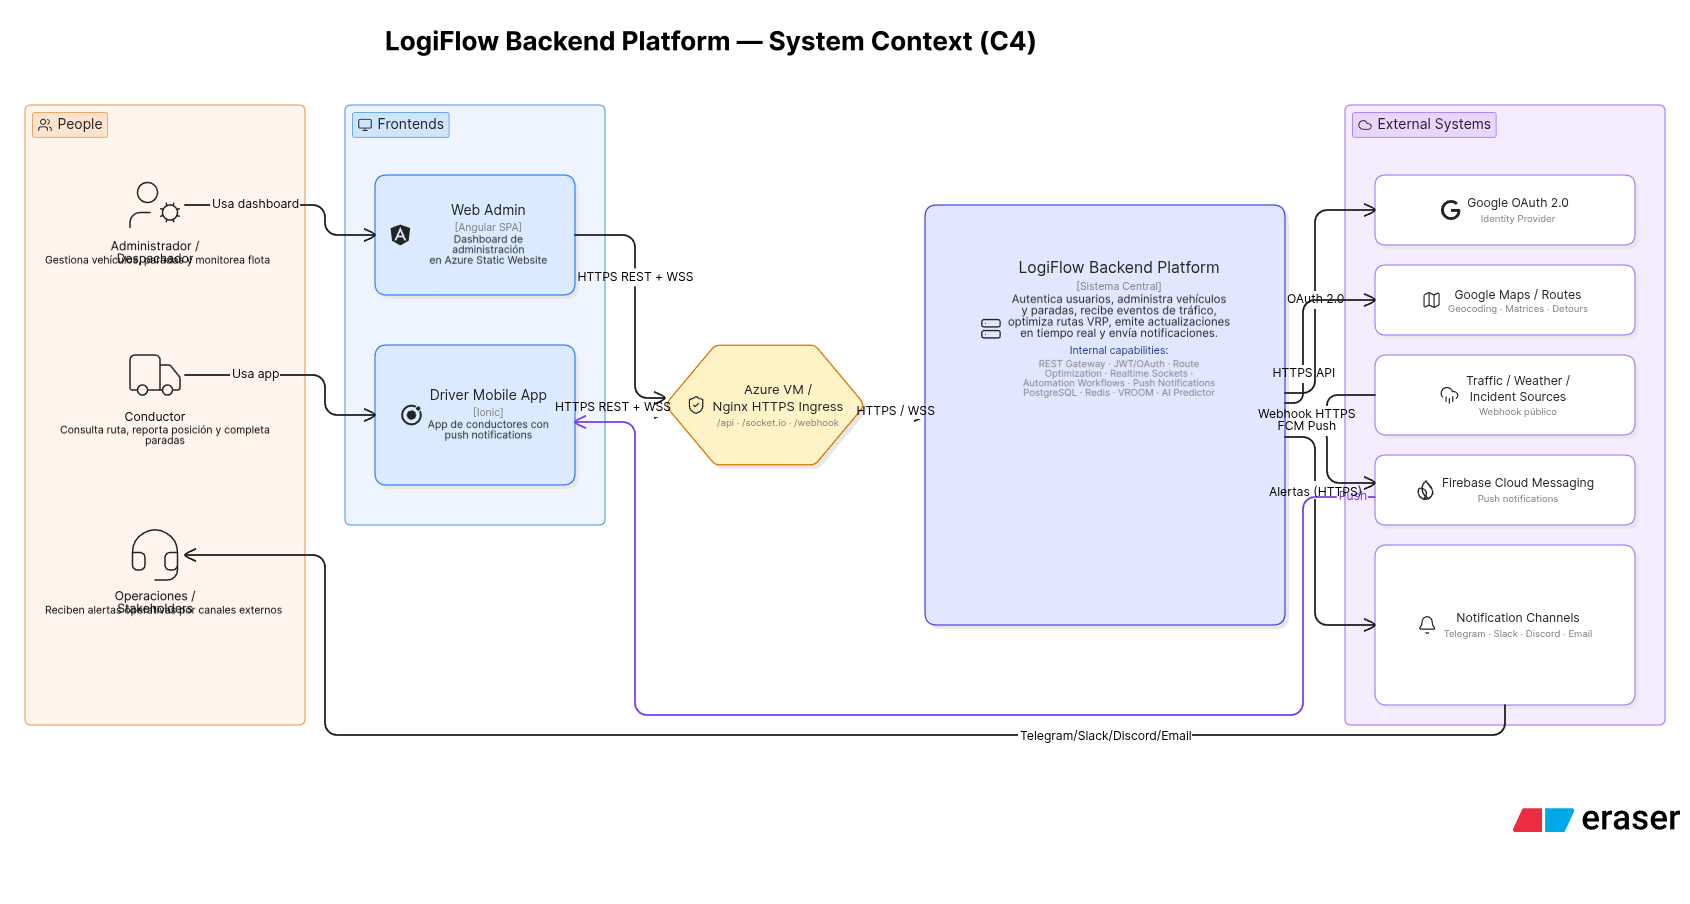
\includegraphics[width=0.95\textwidth]{diagrams/01-context.png}
\caption{Diagrama de Contexto --- LogiFlow Backend Platform y sus actores externos}
\label{fig:contexto}
\end{figure}

El sistema interact\'ua con tres tipos de actores humanos (Administrador/Despachador, Conductor, Operaciones/Stakeholders), dos frontends propios (Web Admin Angular, Driver Mobile App Ionic) y cinco sistemas externos (Google OAuth, Google Maps APIs, Firebase Cloud Messaging, canales de notificaci\'on Telegram/Slack/Discord/Email, y fuentes externas de eventos de tr\'afico). El backend completo se representa como una sola caja con la nota interna de capacidades.

\subsection{Diagrama de Componentes (C4 Nivel 2-3)}

\begin{figure}[H]
\centering
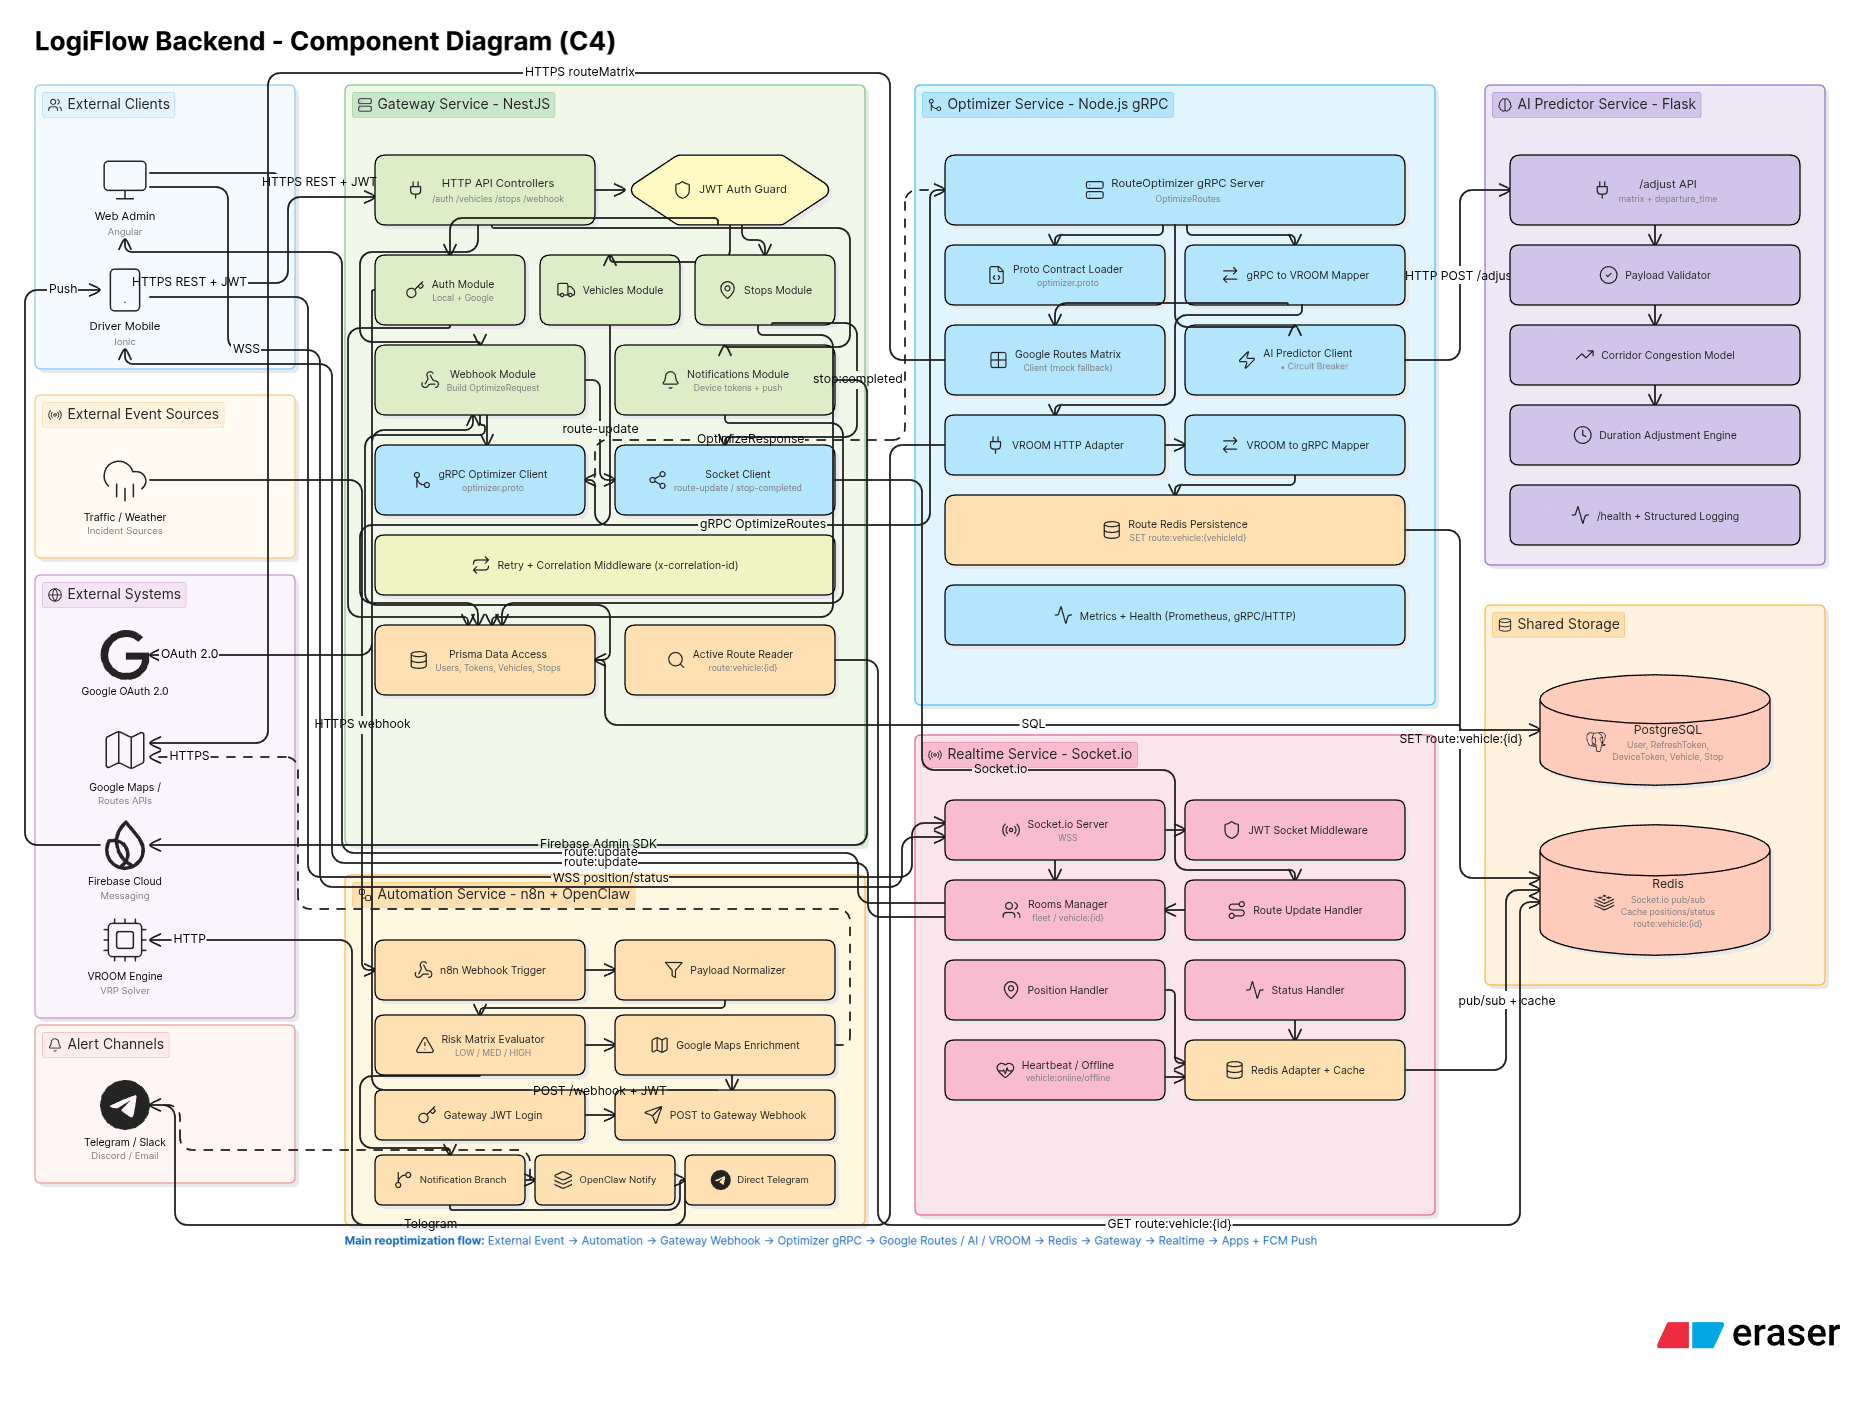
\includegraphics[width=0.95\textwidth]{diagrams/02-components.png}
\caption{Diagrama de Componentes --- 5 servicios backend agrupados con sus componentes internos}
\label{fig:componentes}
\end{figure}

El diagrama muestra los cinco agrupadores principales (Gateway, Optimizer, Realtime, Automation, AI Predictor) con sus componentes internos: controladores HTTP, guards JWT, m\'odulos de auth/vehicles/stops/webhook, cliente gRPC, cliente Socket.io, persistencia Prisma, lector de rutas activas, mapper VROOM, circuit breaker AI, handlers Socket.io, workflows n8n, etc. Se destacan los protocolos entre componentes: HTTPS REST, gRPC, Socket.io, Redis, Prisma/PostgreSQL.

\subsection{Diagrama de Clases}

\begin{figure}[H]
\centering
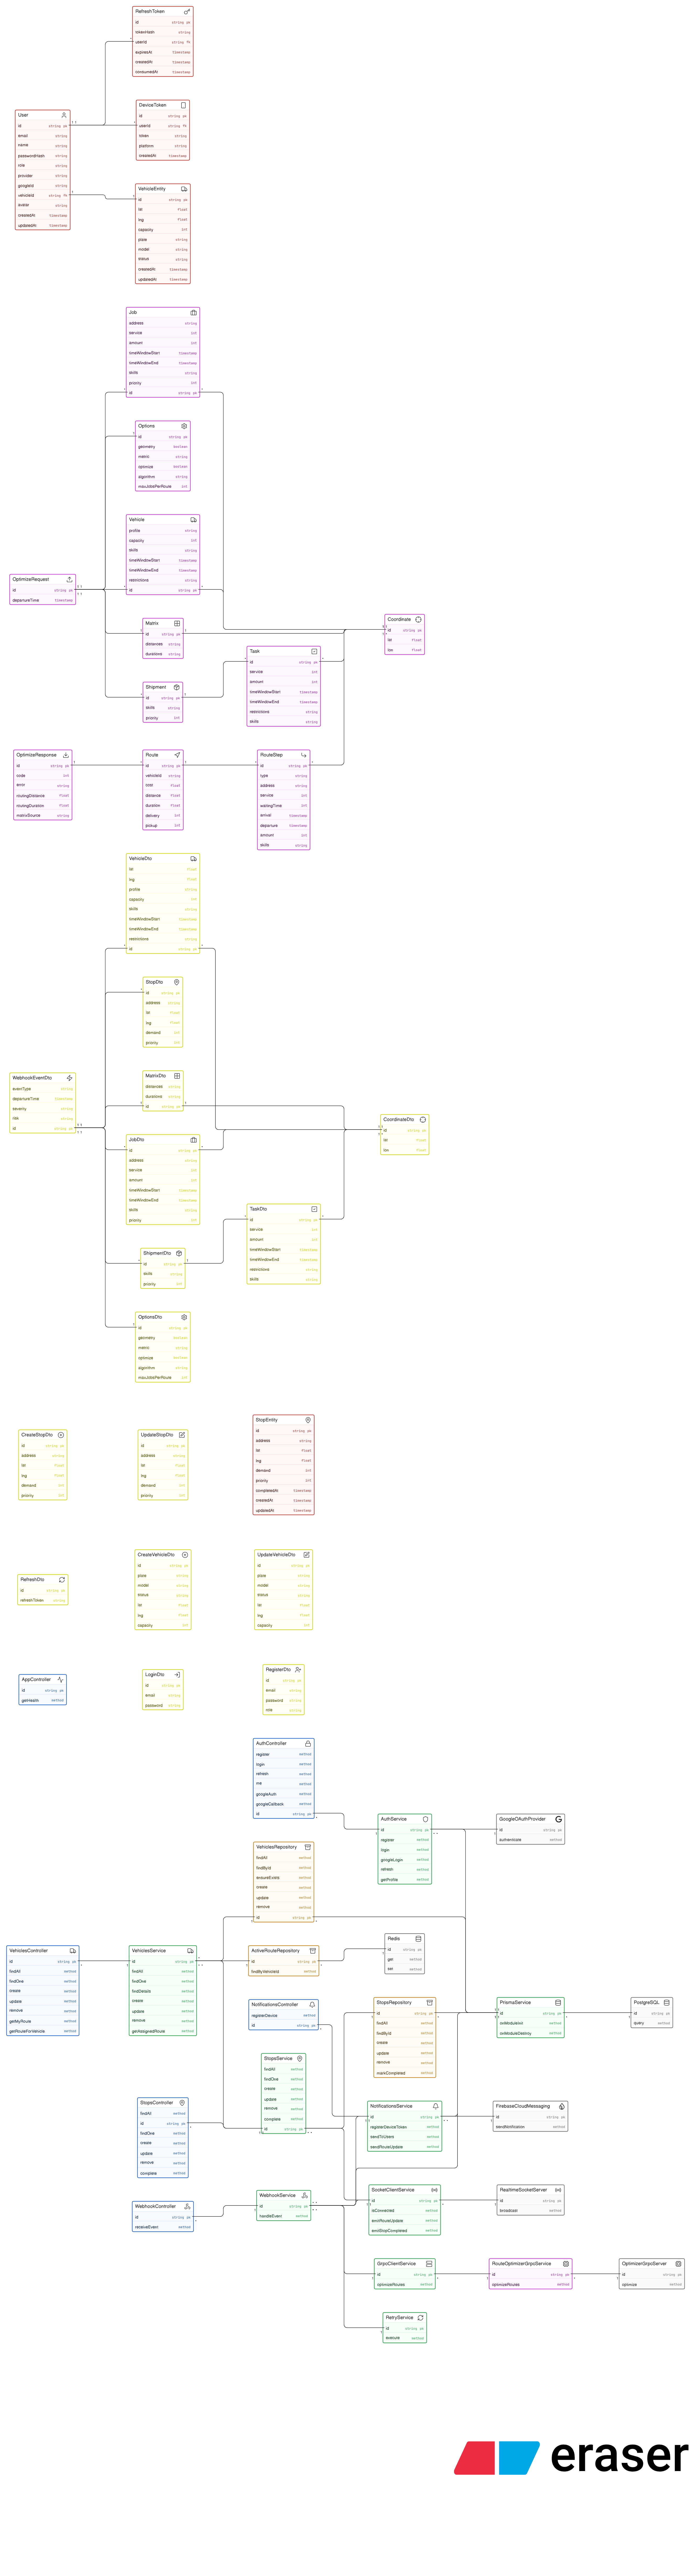
\includegraphics[width=0.95\textwidth]{diagrams/03-classes.png}
\caption{Diagrama de Clases UML --- Controllers, Services, Repositories, DTOs, Entidades del Gateway}
\label{fig:clases}
\end{figure}

Las clases se agrupan en paquetes: \textbf{Controllers} (AuthController, VehiclesController, StopsController, WebhookController, NotificationsController), \textbf{Services} (AuthService, VehiclesService, WebhookService, GrpcClientService, SocketClientService, NotificationsService, RetryService, PrismaService), \textbf{Repositories} (VehiclesRepository, StopsRepository, ActiveRouteRepository), \textbf{DTOs} (LoginDto, WebhookEventDto, VehicleDto, StopDto, etc.), \textbf{gRPC Contract} (RouteOptimizerGrpcService y mensajes Proto3), y \textbf{Persistence Models} (User, RefreshToken, DeviceToken, Vehicle, Stop).

\subsection{Diagrama Entidad-Relaci\'on}

\begin{figure}[H]
\centering
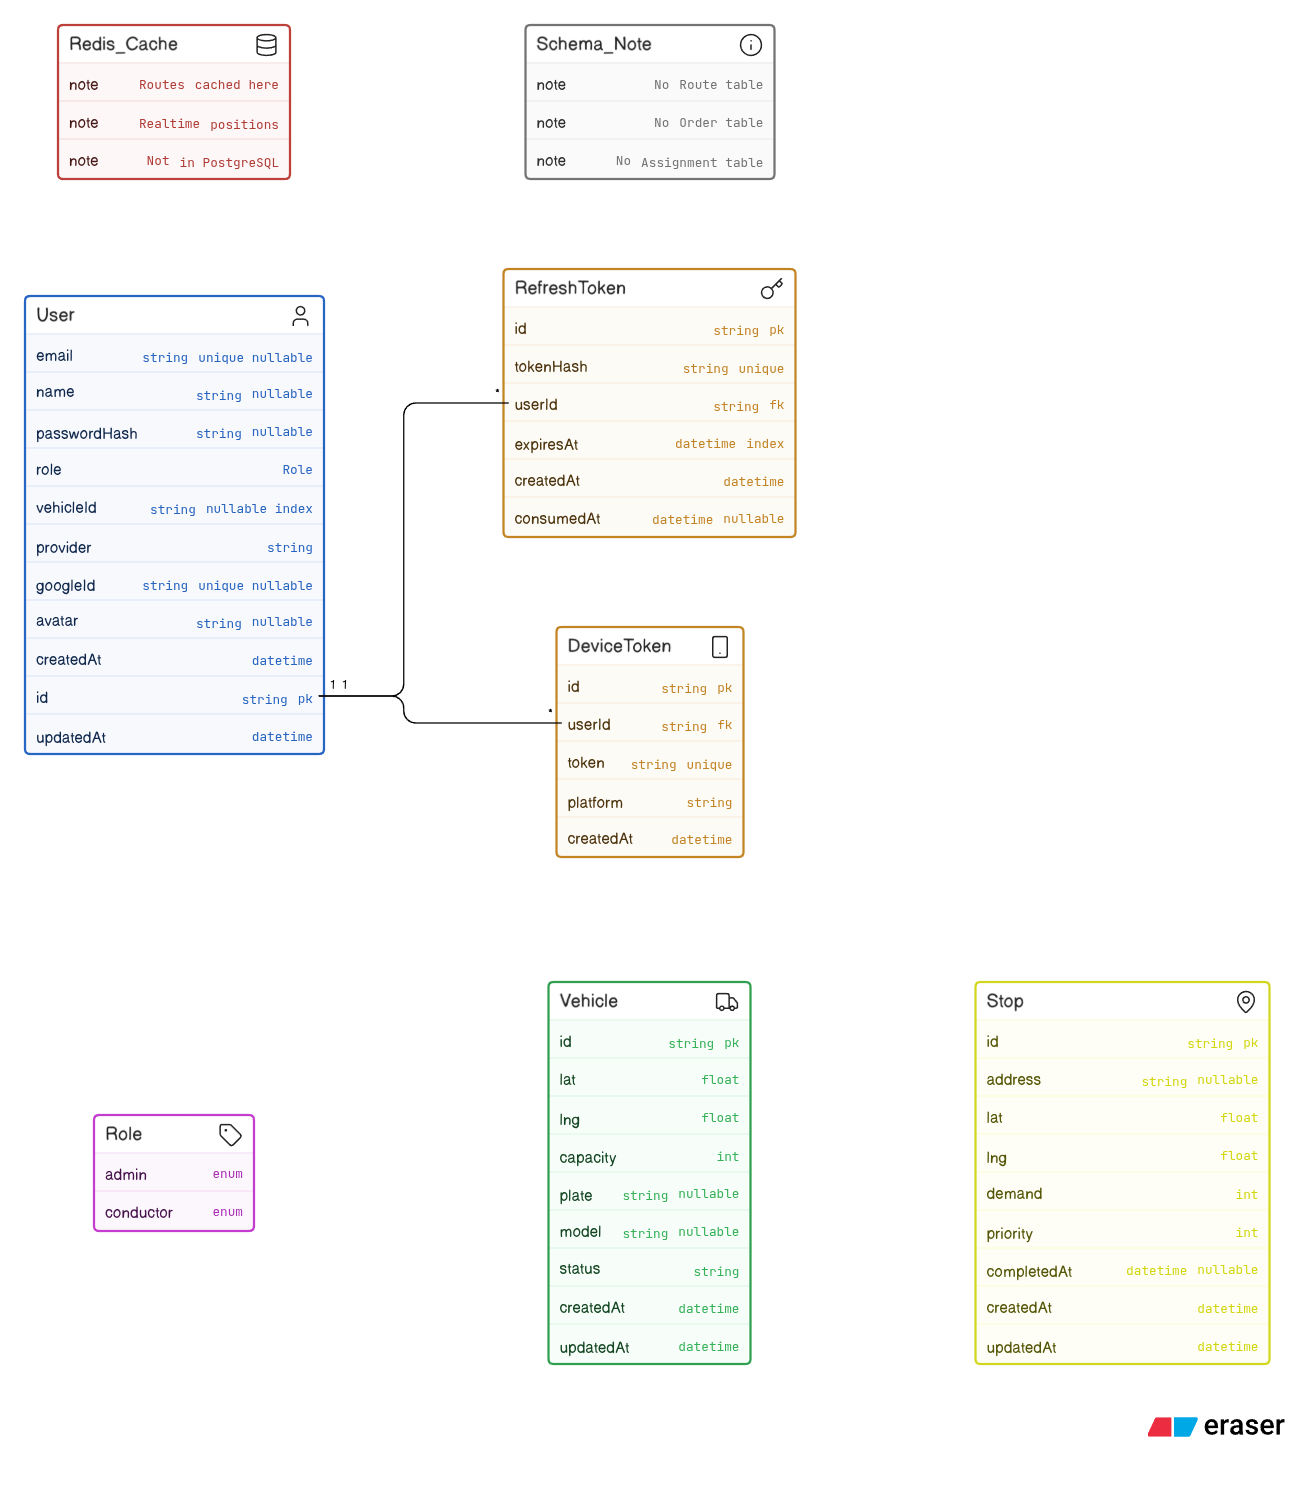
\includegraphics[width=0.85\textwidth]{diagrams/04-er.png}
\caption{Diagrama ER --- Modelo PostgreSQL gestionado por Prisma}
\label{fig:er}
\end{figure}

El esquema PostgreSQL contiene 5 entidades principales: \textbf{User} (con enum Role: admin/conductor), \textbf{RefreshToken} (1:N desde User, cascade delete, con \texttt{consumedAt} para detecci\'on de reuso), \textbf{DeviceToken} (1:N desde User), \textbf{Vehicle} y \textbf{Stop} (entidades operativas independientes). La relaci\'on User-Vehicle es \emph{l\'ogica no estricta} (asignaci\'on por \texttt{vehicleId} sin FK enforced). \textbf{Nota cr\'itica:} las rutas activas no se almacenan en PostgreSQL; se cachean en Redis bajo \texttt{route:vehicle:\{vehicleId\}}.

\subsection{Diagrama de Secuencia --- Reoptimizaci\'on por evento de tr\'afico}

\begin{figure}[H]
\centering
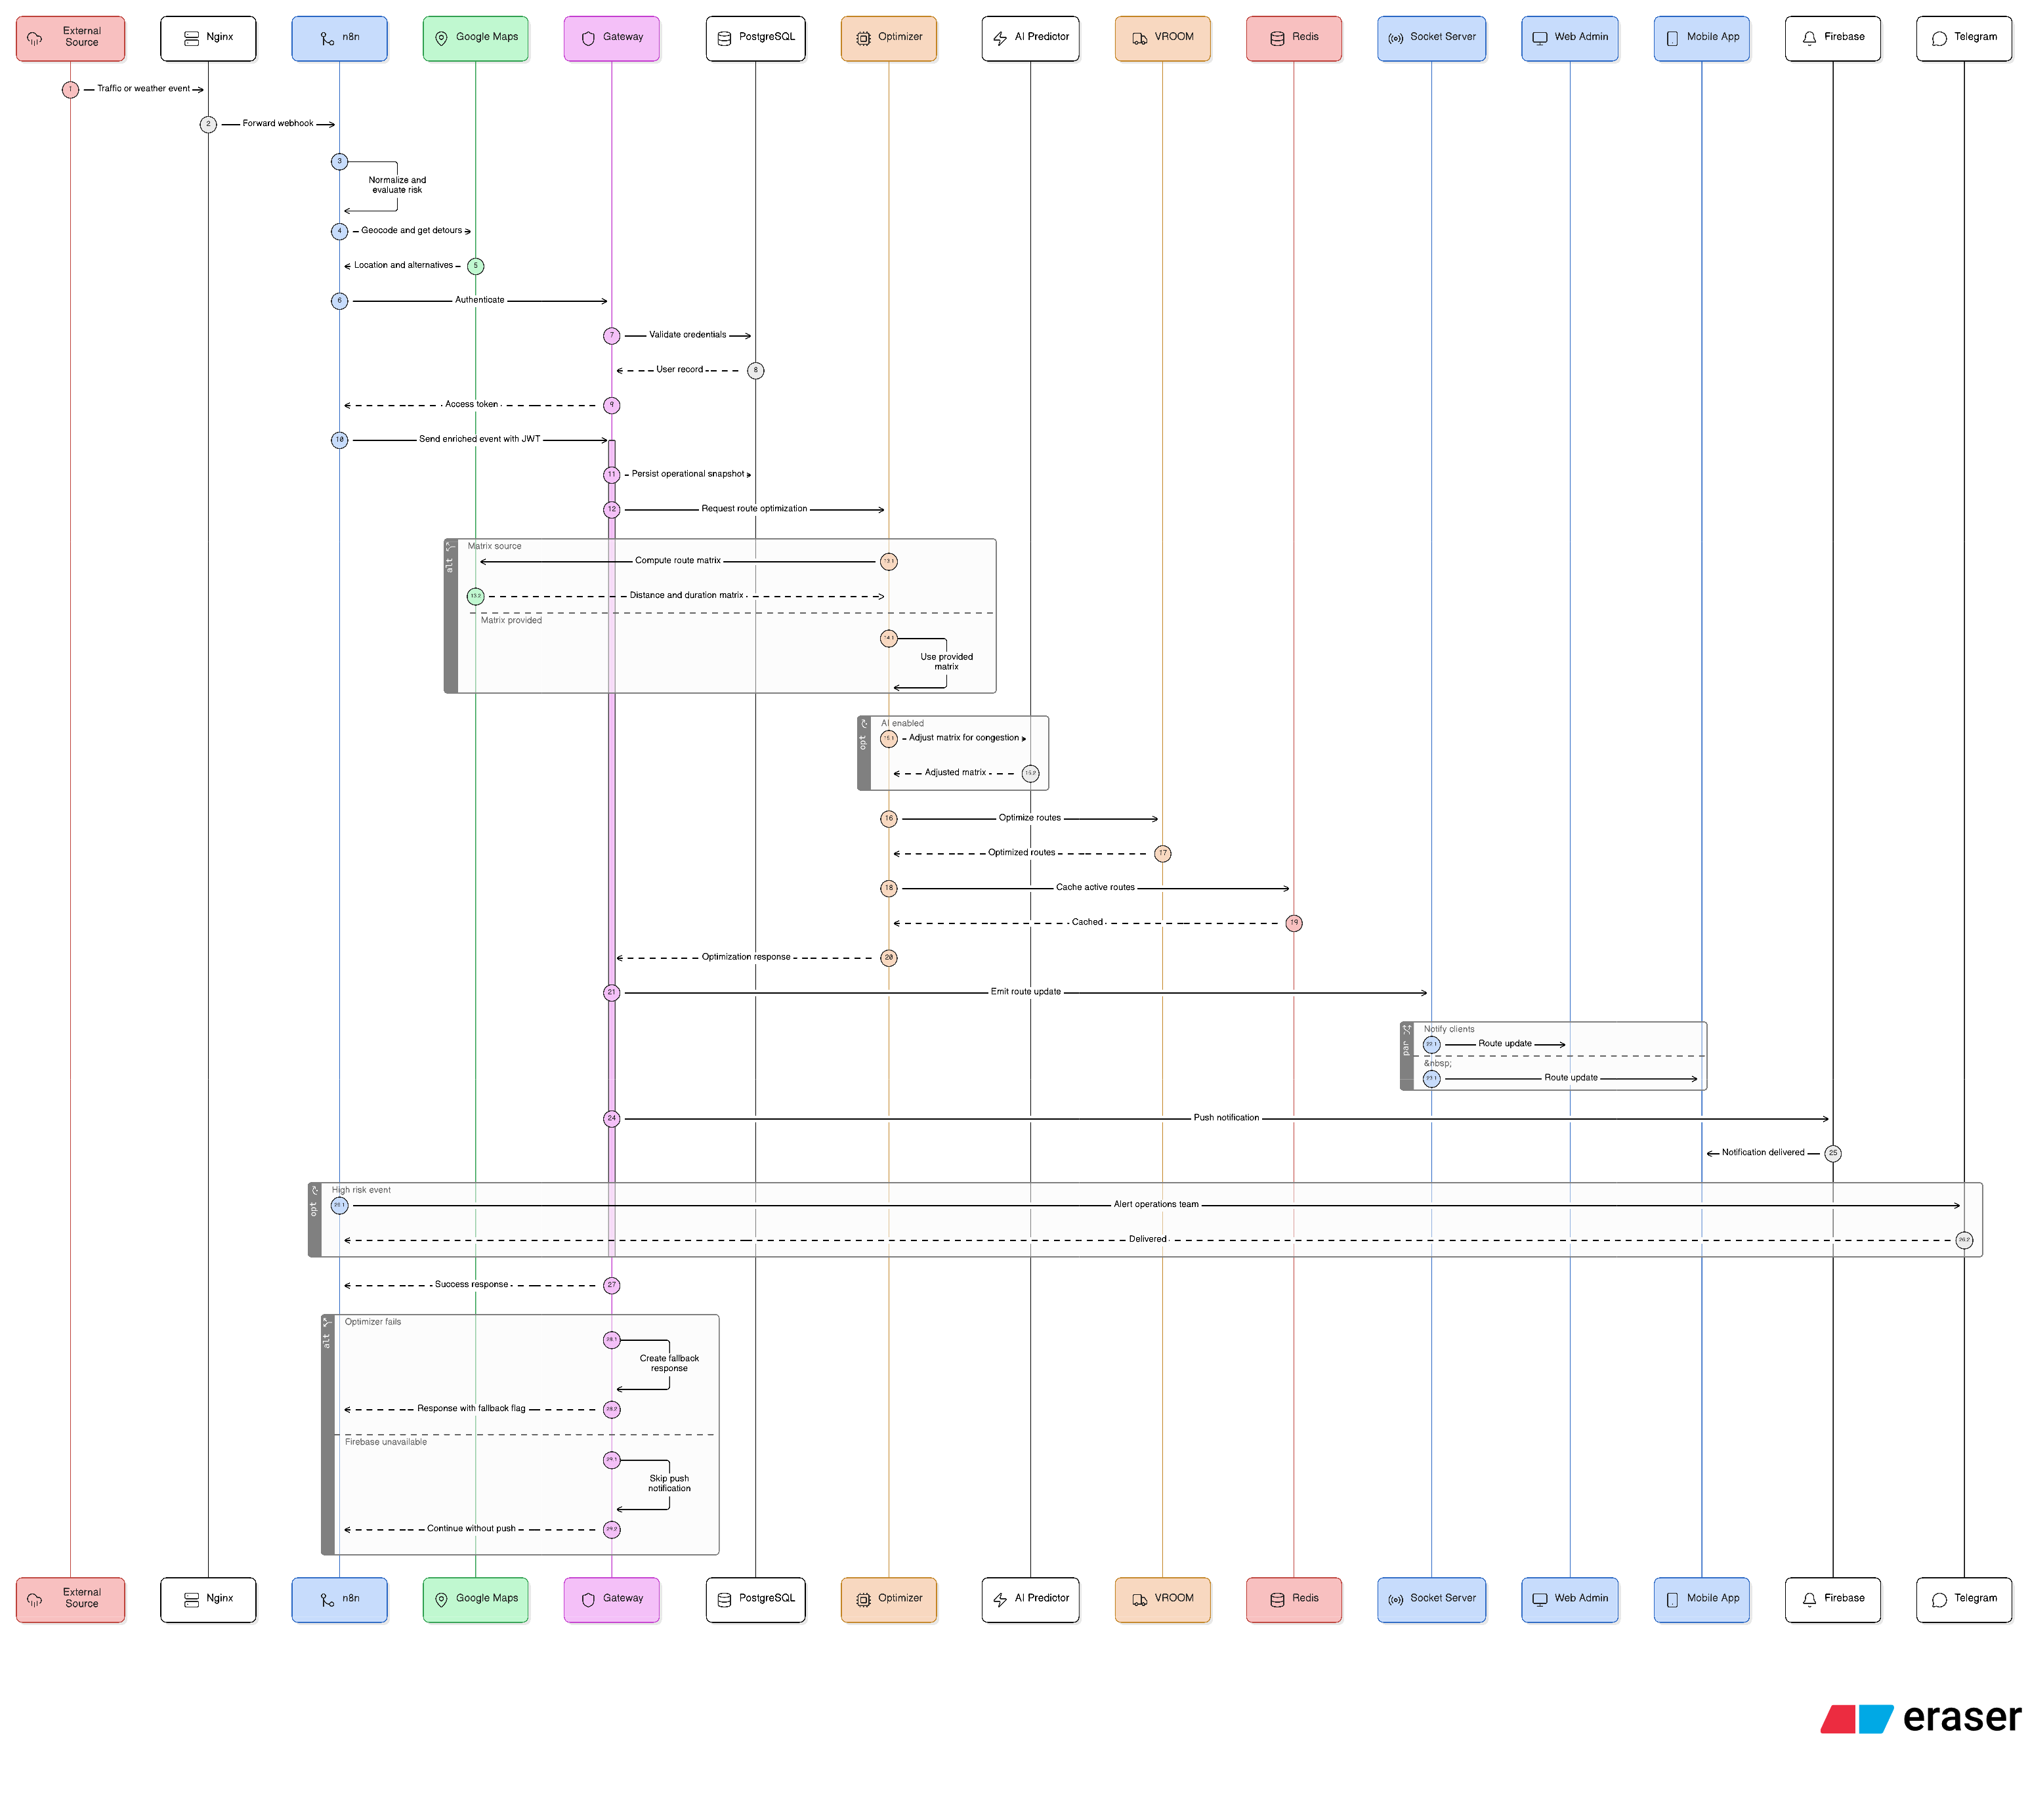
\includegraphics[width=0.95\textwidth]{diagrams/05-sequence.png}
\caption{Diagrama de Secuencia --- Flujo end-to-end de reoptimizaci\'on disparada por evento externo}
\label{fig:secuencia}
\end{figure}

El flujo cubre 19 pasos principales: (1) evento externo llega al webhook p\'ublico, (2) Nginx ru\-te\-a a n8n, (3-5) n8n normaliza, eval\'ua riesgo y enriquece con Google Maps, (6) n8n autentica contra el Gateway con JWT, (7) Gateway recibe el evento y persiste snapshot, (8-10) Gateway invoca al Optimizer v\'ia gRPC, (11-13) Optimizer prepara matriz (Google Routes / AI Predictor / cached) y llama a VROOM, (14) Optimizer persiste rutas en Redis, (15) Gateway recibe rutas, (16-17) Gateway emite \texttt{route:update} v\'ia Socket.io a rooms \texttt{fleet} y \texttt{vehicle:<id>}, (18) Gateway env\'ia push v\'ia Firebase, (19) n8n env\'ia alerta opcional si el riesgo es alto.

Se incluyen bloques alternos para fallback cuando Optimizer, AI Predictor, Google Routes, Firebase o Socket.io fallan.

\subsection{Diagrama de Despliegue}

\begin{figure}[H]
\centering
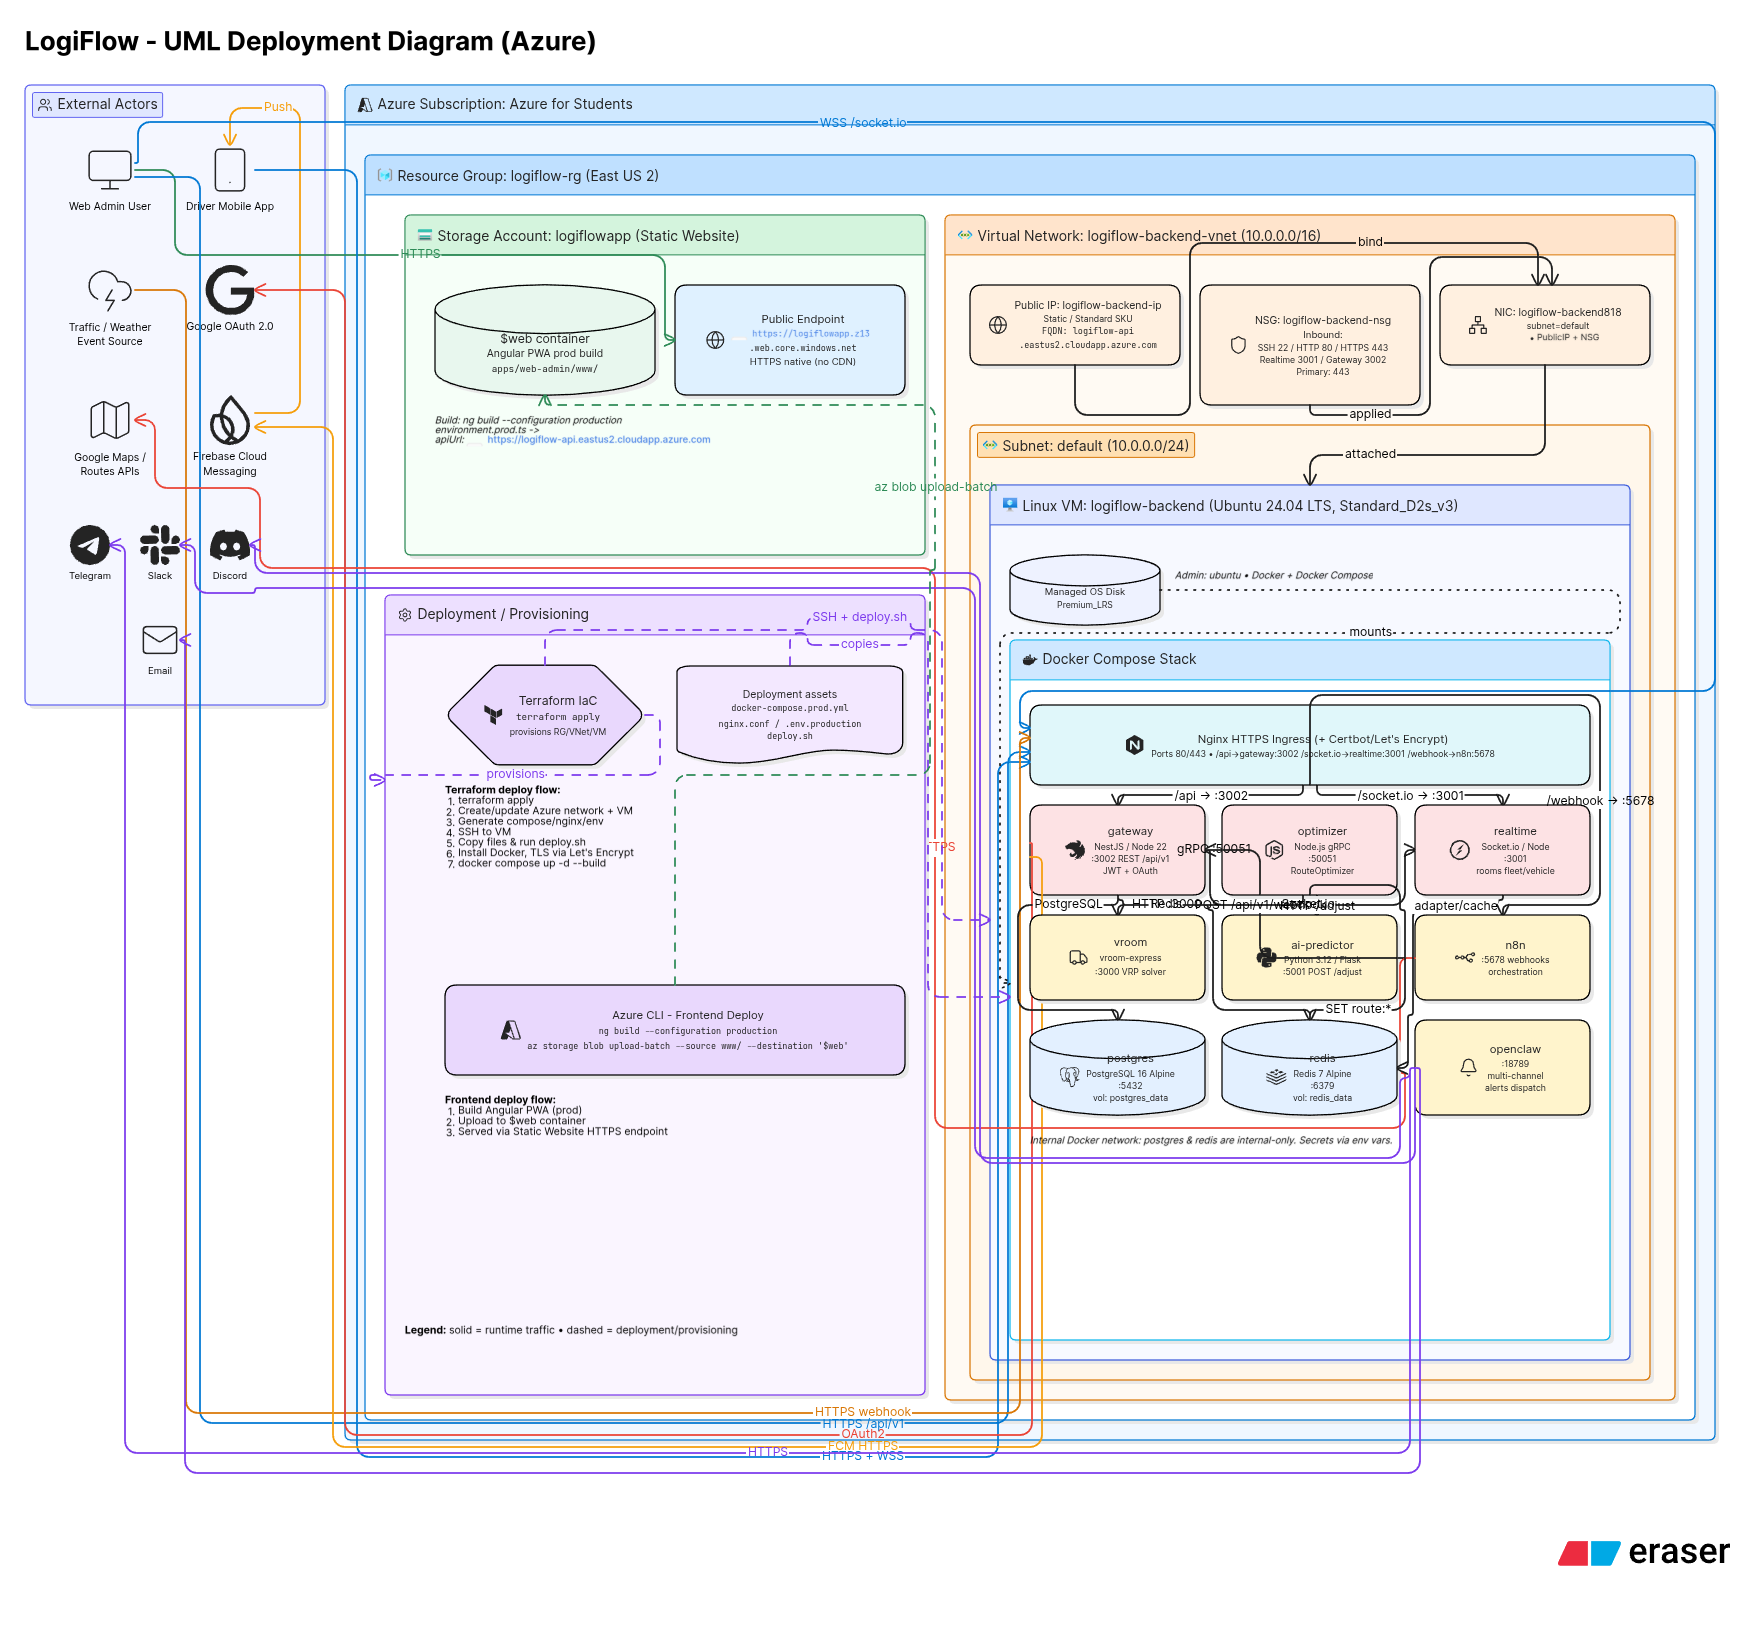
\includegraphics[width=0.95\textwidth]{diagrams/06-deployment.png}
\caption{Diagrama de Despliegue --- Azure Subscription, Resource Group, VM y Docker Compose stack}
\label{fig:despliegue}
\end{figure}

El diagrama representa:
\begin{itemize}[leftmargin=*]
  \item \textbf{Azure Storage Account} \texttt{logiflowapp} sirviendo la PWA Angular desde el contenedor \texttt{\$web} v\'ia HTTPS nativo en \texttt{logiflowapp.z13.web.core.windows.net}.
  \item \textbf{Resource Group} \texttt{logiflow-rg} con VNet, Subnet, Public IP est\'atico, NSG y NIC asociados.
  \item \textbf{Linux VM} \texttt{logiflow-backend} (Standard\_D2s\_v3, Ubuntu 24.04) ejecutando el stack Docker Compose con Nginx + Certbot + gateway + optimizer + vroom + ai-predictor + realtime + postgres + redis + n8n + openclaw.
  \item \textbf{Terraform} provisiona y mantiene toda la infraestructura Azure.
  \item Servicios externos: Google OAuth, Google Maps APIs, Firebase Cloud Messaging, canales de notificaci\'on.
\end{itemize}

\subsection{Diagrama de Actividades}

\begin{figure}[H]
\centering
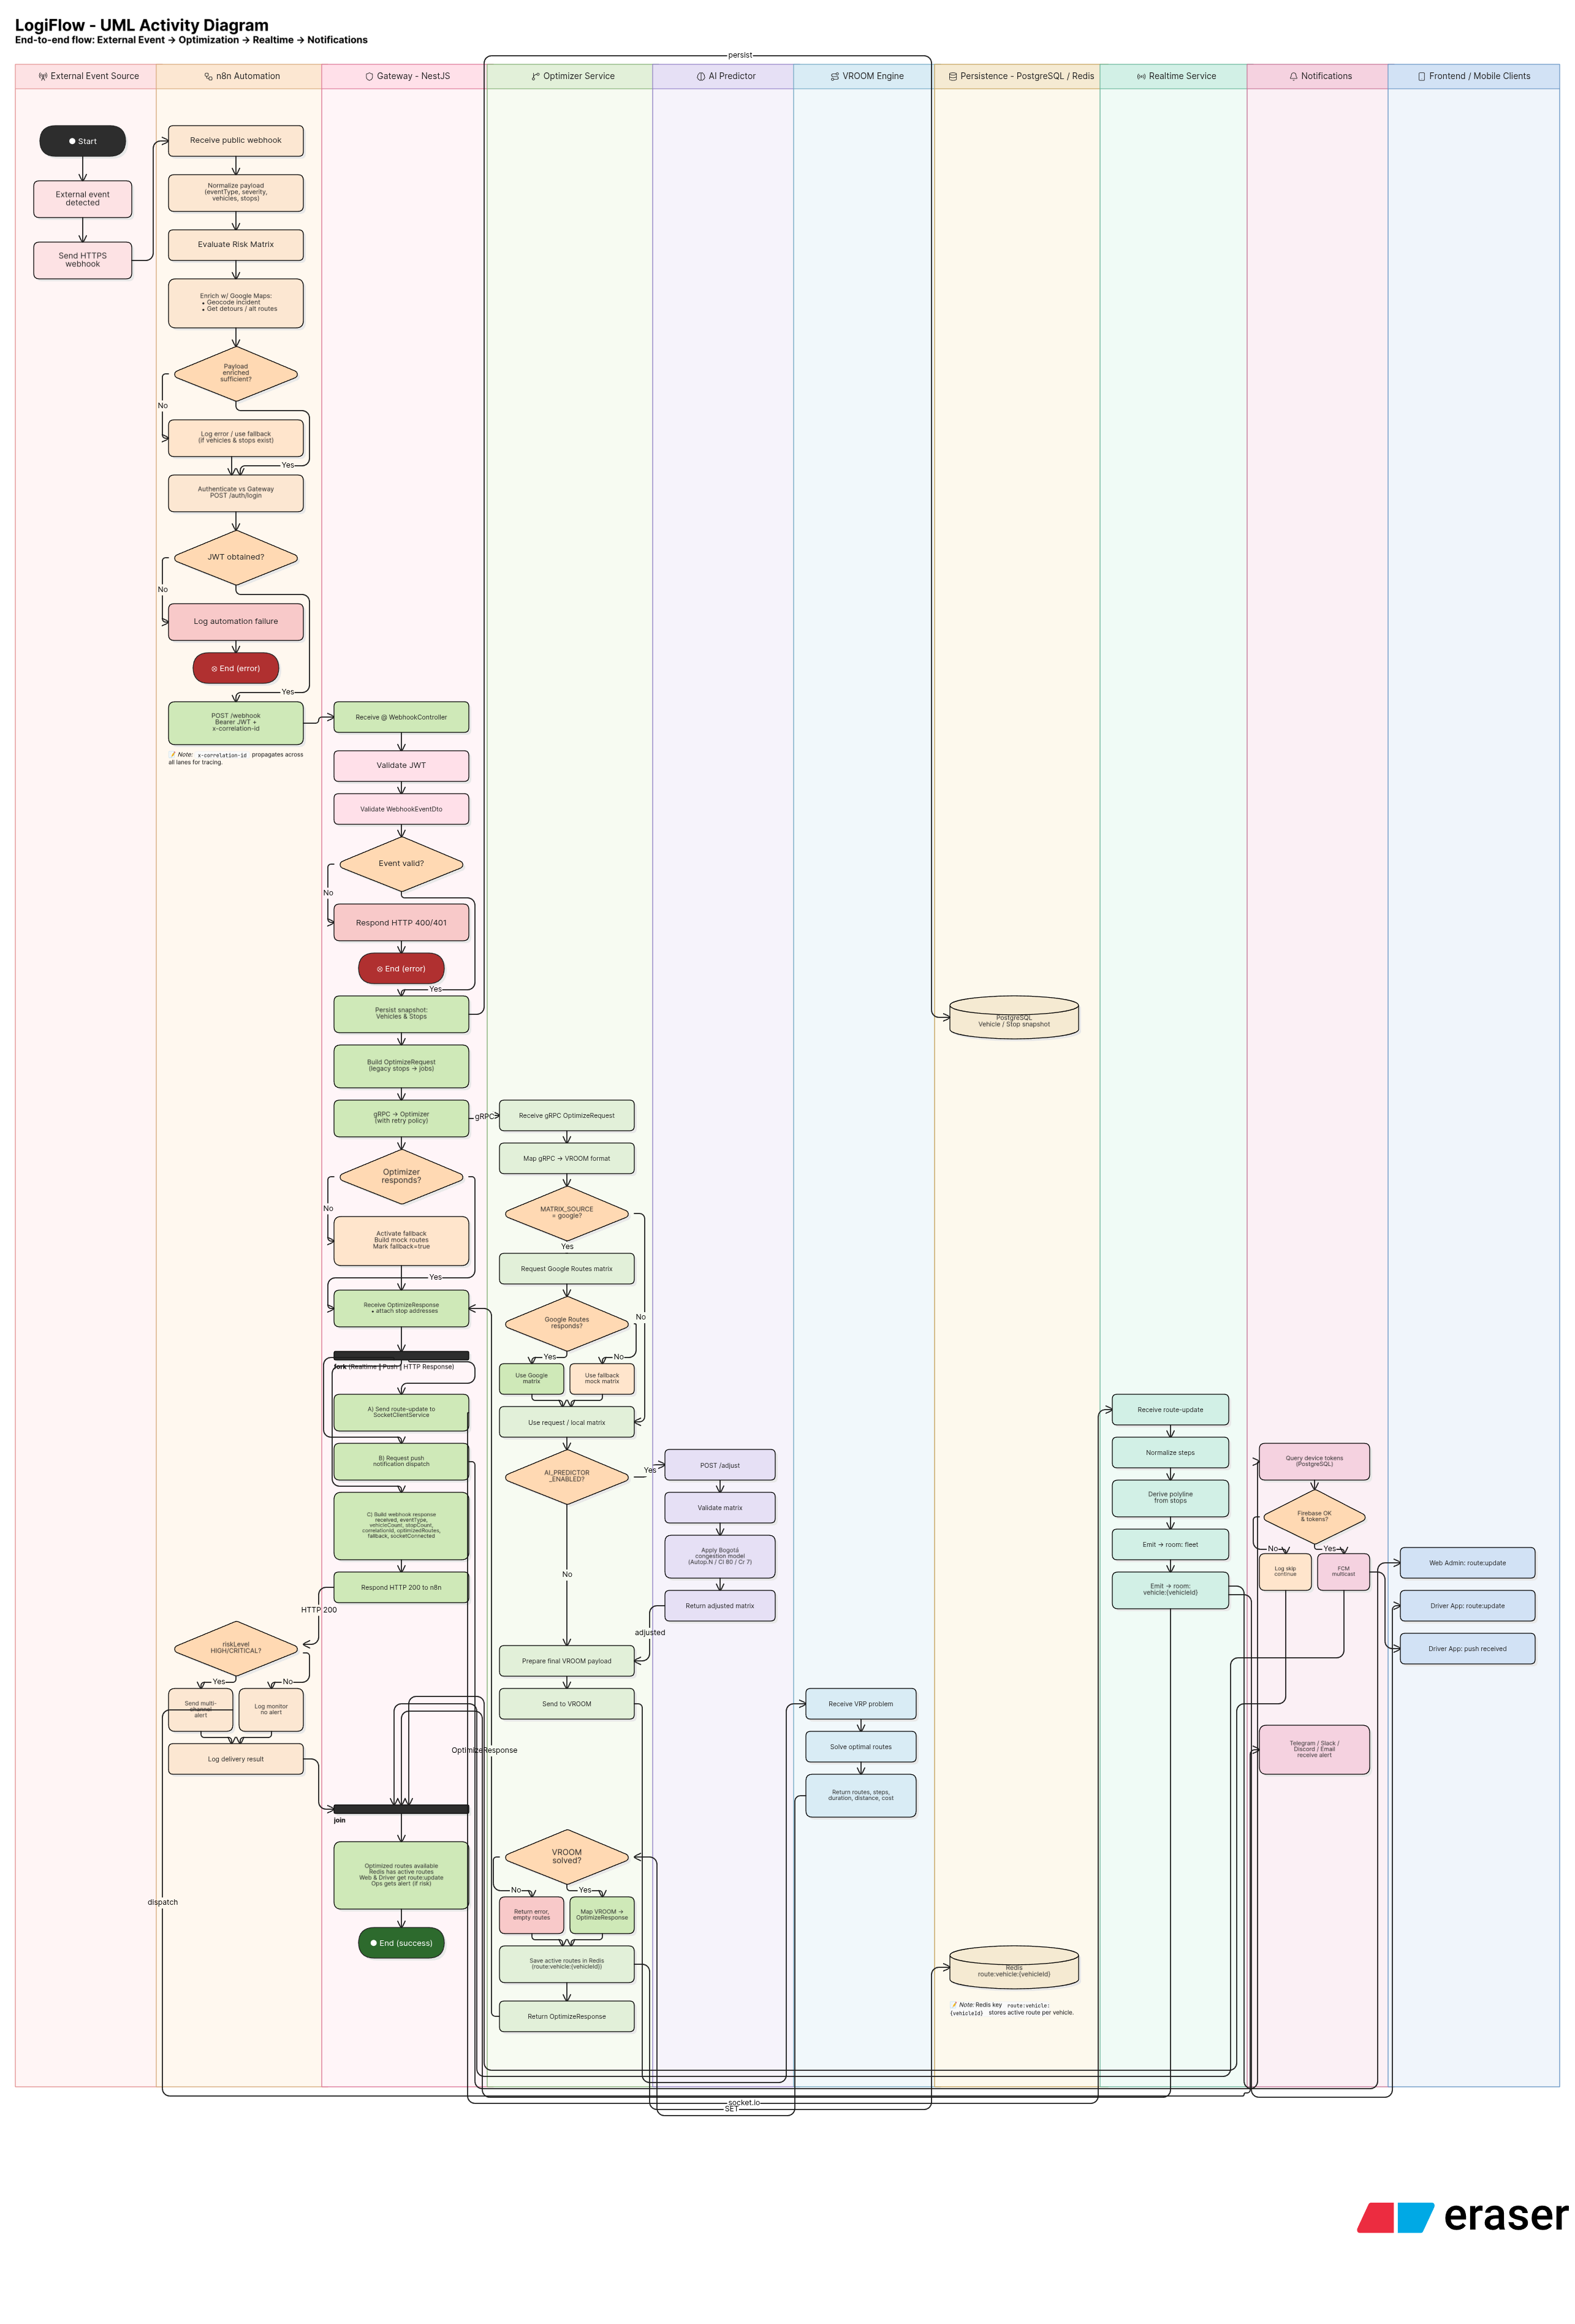
\includegraphics[width=0.95\textwidth]{diagrams/07-activity.png}
\caption{Diagrama de Actividades --- Procesamiento de evento de tr\'afico con swimlanes por responsable}
\label{fig:actividades}
\end{figure}

El diagrama de actividades muestra el flujo con 10 swimlanes (External Event Source, n8n Automation, Gateway, Optimizer, AI Predictor, VROOM, Persistence, Realtime, Notifications, Frontend/Mobile Clients) y los puntos de decisi\'on principales: validaci\'on de payload, evaluaci\'on de risk matrix, selecci\'on de \texttt{MATRIX\_SOURCE}, decisi\'on de habilitar AI Predictor, manejo de fallbacks de VROOM/Optimizer/Firebase y env\'io condicional de alertas.

% =============================================================================
%  7. DETALLES TECNOLOGICOS
% =============================================================================
\section{Detalles Tecnol\'ogicos}

\subsection{Lenguajes y frameworks}

\begin{table}[H]
\centering
\caption{Stack tecnol\'ogico por servicio}
\label{tab:stack}
\small
\begin{tabularx}{\textwidth}{p{3cm} p{3.5cm} X}
\toprule
\textbf{Servicio} & \textbf{Lenguaje / Runtime} & \textbf{Frameworks y librer\'ias clave} \\
\midrule
gateway & TypeScript 5.7 / Node.js 22 & NestJS 11, Prisma 7, \texttt{@grpc/grpc-js}, \texttt{passport-google-oauth20}, \texttt{passport-jwt}, \texttt{firebase-admin}, \texttt{socket.io-client}, bcrypt, Swagger \\
realtime & JavaScript / Node.js 22 & socket.io 4.8, \texttt{@socket.io/redis-adapter}, express 5, ioredis, jsonwebtoken \\
optimizer & JavaScript / Node.js 22 & \texttt{@grpc/grpc-js}, \texttt{@grpc/proto-loader}, axios, ioredis, opossum (circuit breaker), pino (JSON logging), prom-client (Prometheus) \\
ai-predictor & Python 3.12 & Flask 3.1, gunicorn 23, structlog 24 \\
vroom & C++ & VROOM (motor VRP), vroom-express \\
automation (n8n) & JavaScript / Node.js & n8n 1.66.0 (pinned) \\
automation (openclaw) & JavaScript / Node.js & OpenClaw 2026.5.12-slim, Anthropic SDK (Claude Sonnet 4) \\
\midrule
web-admin & TypeScript 5.9 & Angular 20, Ionic 8 (componentes), Google Maps JS API \\
mobile & TypeScript 5.x & Angular 20, Ionic 8, Capacitor 8 (\texttt{@capacitor/geolocation}, \texttt{@capacitor/push-notifications}, \texttt{@capacitor/preferences}) \\
\bottomrule
\end{tabularx}
\end{table}

\subsection{Infraestructura y servicios}

\begin{itemize}[leftmargin=*]
  \item \textbf{Cloud:} Microsoft Azure (Azure for Students subscription) --- regi\'on East US 2.
  \item \textbf{Compute:} Azure Virtual Machine Standard\_D2s\_v3 (2 vCPUs, 8 GB RAM, Ubuntu Server 24.04 LTS).
  \item \textbf{Storage:} Azure Blob Storage con Static Website habilitado (contenedor \texttt{\$web}).
  \item \textbf{Networking:} VNet \texttt{logiflow-backend-vnet} (10.0.0.0/16), Subnet \texttt{default} (10.0.0.0/24), Public IP Standard SKU, NSG con reglas inbound para 22 (SSH), 80, 443, 3001, 3002.
  \item \textbf{DNS:} FQDN gratuito de Azure: \texttt{logiflow-api.eastus2.cloudapp.azure.com}.
  \item \textbf{TLS:} Let's Encrypt v\'ia Certbot, renovaci\'on autom\'atica cada 12 horas.
  \item \textbf{Reverse proxy:} Nginx con rutas \texttt{/api/*} $\rightarrow$ gateway:3002, \texttt{/socket.io/*} $\rightarrow$ realtime:3001, \texttt{/webhook/*} $\rightarrow$ n8n:5678.
  \item \textbf{Base de datos:} PostgreSQL 16 Alpine dentro de Docker con volumen persistente \texttt{postgres\_data}.
  \item \textbf{Cache / broker:} Redis 7 Alpine con autenticaci\'on por password en producci\'on (\texttt{--requirepass}).
  \item \textbf{IaC:} Terraform con dos m\'odulos: \texttt{network} (VNet, Subnet, Public IP, NSG) y \texttt{vm} (VM Linux + OS Disk + NIC).
\end{itemize}

\subsection{DevOps y CI/CD}

\subsubsection{Pipeline CI --- Backend}

GitHub Actions con estrategia matrix para los cuatro servicios principales:

\begin{lstlisting}[caption={Workflow CI del backend (.github/workflows/ci.yml)}]
strategy:
  matrix:
    service: [automation, gateway, realtime, optimizer]
  fail-fast: false
steps:
  - uses: actions/checkout@v4
  - uses: actions/setup-node@v4
    with: { node-version: 20 }
  - run: npm ci
  - run: npx prisma generate    # solo gateway
  - run: npm run lint
  - run: npm test -- --coverage --coverageReporters=lcov --passWithNoTests
  - uses: SonarSource/sonarcloud-github-action@master   # si existe sonar-project.properties
\end{lstlisting}

\subsubsection{Pipeline CD --- Backend}

Trigger: \texttt{workflow\_run} despu\'es de CI exitoso sobre \texttt{main}, o \texttt{workflow\_dispatch} manual.

\begin{enumerate}[leftmargin=*]
  \item Checkout del c\'odigo.
  \item Configuraci\'on de clave SSH desde secreto \texttt{SSH\_PRIVATE\_KEY} (base64-encoded).
  \item \texttt{rsync} de fuente a la VM en \texttt{/home/ubuntu/logiflow} (excluye \texttt{.git}, \texttt{node\_modules}, \texttt{dist}, \texttt{*.log}, \texttt{infra/generated}).
  \item SSH a la VM y ejecuci\'on: \texttt{docker-compose -f docker-compose.prod.yml up -d --build --remove-orphans}.
  \item Smoke test: \texttt{curl} a \texttt{https://logiflow-api.eastus2.cloudapp.azure.com/api/v1} hasta 8 veces con 15s de intervalo (200/401/404 pasan).
\end{enumerate}

\subsubsection{Pipeline CI/CD --- Frontend}

\textbf{CI:} \texttt{npm run typecheck} (tsc -b cruzando apps + libs) + \texttt{npm run lint -w @logiflow/web-admin}.

\textbf{CD (solo web-admin):} \texttt{ng build --configuration production} con inyecci\'on de env vars v\'ia \texttt{set-env.js}, luego \texttt{az storage blob upload-batch} al contenedor \texttt{\$web} del Storage Account.

\textbf{Mobile:} no tiene pipeline de despliegue autom\'atico. El APK Android se genera localmente con \texttt{npm run build:android} + \texttt{npx cap open android} y se distribuye manualmente.

% =============================================================================
%  8. SEGURIDAD DEL SISTEMA
% =============================================================================
\section{Seguridad del Sistema}

\subsection{Autenticaci\'on y autorizaci\'on}

\paragraph{M\'etodo \'unico de autenticaci\'on.} Tras la migraci\'on completada en el Sprint 8-10, el sistema soporta \emph{exclusivamente} Google OAuth 2.0. No existen endpoints de registro local ni login por usuario/contrase\~na. La p\'agina de login en ambos frontends solo muestra el bot\'on ``Continue with Google''.

\paragraph{Flujo de autenticaci\'on web (Authorization Code).}
\begin{enumerate}[leftmargin=*]
  \item Frontend redirige a \texttt{GET /api/v1/auth/google?app=admin|mobile|web}.
  \item Backend (passport-google-oauth20) redirige a Google consent screen.
  \item Tras consentimiento, Google redirige a \texttt{GET /api/v1/auth/google/callback}.
  \item Backend hace upsert del usuario en PostgreSQL (rol \texttt{admin} si el email est\'a en \texttt{GOOGLE\_ADMIN\_EMAILS}, sino \texttt{conductor}).
  \item Backend genera JWT (1h) y refresh token (7 d\'ias, hash SHA-256).
  \item Backend redirige al frontend con \texttt{?accessToken=...\&refreshToken=...\&role=...} (la URL del frontend depende del par\'ametro \texttt{?app=} original).
\end{enumerate}

\paragraph{Flujo de autenticaci\'on m\'ovil (ID Token Exchange).}
La app m\'ovil puede obtener el Google ID Token v\'ia el SDK nativo de Google Sign-In y enviarlo a \texttt{POST /api/v1/auth/google/token}. El backend valida el token con \texttt{google-auth-library} (verifyIdToken con \texttt{GOOGLE\_CLIENT\_ID} como audience) y devuelve directamente el JWT del sistema.

\paragraph{Autorizaci\'on por rol.}
\begin{itemize}[leftmargin=*]
  \item Frontend: \texttt{AuthGuard} de Angular decodifica el JWT desde \texttt{localStorage}, extrae \texttt{role} y redirige al login si no coincide con el rol esperado por la ruta.
  \item Backend: \texttt{JwtAuthGuard} de NestJS protege todos los endpoints REST sensibles; las operaciones de webhook y CRUD de flota requieren rol \texttt{admin}.
  \item WebSocket: \texttt{io.use()} middleware valida el JWT del handshake, decodifica claims y une el socket a la room apropiada (\texttt{fleet} para admin, \texttt{vehicle:<vehicleId>} para conductor).
\end{itemize}

\subsection{Cifrado}

\begin{itemize}[leftmargin=*]
  \item \textbf{En tr\'ansito p\'ublico:} TLS 1.2/1.3 v\'ia Let's Encrypt en Nginx (\texttt{logiflow-api.eastus2.cloudapp.azure.com}) y v\'ia certificado nativo de Azure en el Storage Account (\texttt{logiflowapp.z13.web.core.windows.net}).
  \item \textbf{WebSocket:} WSS sobre el mismo certificado Let's Encrypt.
  \item \textbf{En tr\'ansito interno:} comunicaci\'on entre contenedores Docker es HTTP plano dentro de la red \texttt{logiflow-prod} (no expuesta al exterior). gRPC entre Gateway y Optimizer tambi\'en es HTTP/2 plano internamente.
  \item \textbf{En reposo:}
  \begin{itemize}
    \item Refresh tokens almacenados como hash SHA-256.
    \item Passwords (hist\'oricos, antes de migraci\'on a Google OAuth) hash bcrypt salt rounds 10.
    \item Firebase private key, JWT secret y Google client secret almacenados como variables de entorno; nunca commiteados al repositorio.
    \item Redis configurado con \texttt{--requirepass} en producci\'on.
  \end{itemize}
\end{itemize}

\subsection{Buenas pr\'acticas}

\begin{enumerate}[leftmargin=*]
  \item \textbf{No logging de informaci\'on sensible.} El logger del Gateway redacta JWT y refresh tokens.
  \item \textbf{Refresh Token Rotation Single-Use.} Cada refresh token solo puede usarse una vez; se marca \texttt{consumedAt} en la primera consumici\'on y se invalida.
  \item \textbf{Correlation ID propagado.} Cada request entrante recibe (o genera) un \texttt{x-correlation-id} que se propaga a logs, llamadas gRPC, eventos Socket.io y notificaciones. Permite trazar un evento end-to-end en producci\'on.
  \item \textbf{CORS restrictivo.} \texttt{CORS\_ORIGINS} acepta solo los dom\'inios conocidos (Azure Storage frontend, localhost para desarrollo, \texttt{capacitor://localhost} para apps nativas).
  \item \textbf{Helmet en NestJS} (recomendado para activar en pr\'oximo sprint) --- agrega cabeceras de seguridad b\'asicas.
  \item \textbf{Validaci\'on de DTOs con class-validator} en todos los endpoints REST.
  \item \textbf{Sanitizaci\'on de logs} en \texttt{services/automation/mock-server} tras detecci\'on de log injection en CI (commit \texttt{e913ffe}).
  \item \textbf{Secretos en GitHub Secrets} para CI/CD: \texttt{SSH\_PRIVATE\_KEY}, \texttt{SERVER\_IP}, \texttt{SSH\_USER}, \texttt{GOOGLE\_MAPS\_API\_KEY}, \texttt{AZURE\_STORAGE\_ACCOUNT\_KEY}.
\end{enumerate}

% =============================================================================
%  9. BITACORA DE CEREMONIAS
% =============================================================================
\section{Bit\'acora de Ceremonias}

\subsection{Sprint 0 --- Iniciaci\'on (5 pts)}

\textbf{Objetivo:} Establecer infraestructura b\'asica de colaboraci\'on.

\textbf{Entregables:}
\begin{itemize}[leftmargin=*]
  \item Repositorios creados en organizaci\'on \texttt{Logiflow-Gavilanes-ECI}.
  \item Definici\'on inicial del Product Backlog en Azure DevOps.
  \item Branch protection sobre \texttt{main} y \texttt{develop}.
  \item Templates de pull request e issue.
  \item Stack tentativo definido (NestJS + Angular + VROOM).
\end{itemize}

\subsection{Release 1 (Sprints 1-5)}

\subsubsection*{Sprint 1 --- MVP Conectado (13 pts)}
Esqueletos de los 4 servicios principales. Health checks. Docker Compose local funcional. Primer ``Hello World'' end-to-end Gateway $\rightarrow$ Realtime via socket.io.

\subsubsection*{Sprint 2 --- APIs Reales (21 pts)}
CRUD de vehicles y stops. Prisma schema definido. PostgreSQL en Docker. Tests unitarios b\'asicos por servicio (cobertura inicial $\sim$30\%). Swagger UI expuesto en \texttt{/api/v1/docs}.

\subsubsection*{Sprint 3 --- Optimizer Vivo (21 pts)}
Contrato gRPC definido en \texttt{shared/proto/optimizer.proto}. Integraci\'on Gateway $\rightarrow$ Optimizer v\'ia \texttt{@grpc/grpc-js}. Optimizer $\rightarrow$ VROOM v\'ia HTTP. Primer flujo end-to-end de optimizaci\'on con respuesta de rutas reales.

\subsubsection*{Sprint 4 --- Interfaces + Auth (34 pts)}
Frontend Angular Web Admin inicial con login local (JWT). Frontend Mobile Ionic inicial. Mapa Google Maps integrado. Tests E2E b\'asicos. Auth JWT funcional en backend con \texttt{passport-jwt}.

\subsubsection*{Sprint 5 --- Cloud Deploy Azure (Corte 2) (46 pts)}
\textbf{Hito de corte.} Infra Terraform completa: VNet, VM, Public IP, NSG. \texttt{docker-compose.prod.yml} con resource limits. Nginx + Certbot con TLS de Let's Encrypt. GitHub Actions \texttt{deploy-backend.yml} con SSH a la VM. Web Admin desplegado a Azure Storage Static Website. Sistema accesible p\'ublicamente.

\subsection{Release 2 (Sprints 6-10)}

\subsubsection*{Sprint 6 --- Observabilidad + Tests (34 pts)}
Cobertura empujada a $\geq$ 80\% en ambos repos. SonarCloud integrado. Mocks de Prisma para tests del Gateway. Logging estructurado con pino en Optimizer. Refactor de servicios para inyecci\'on de dependencias y testeabilidad.

\subsubsection*{Sprint 7 --- Escala / Performance (21 pts)}
Pruebas de carga con Apache JMeter. Identificaci\'on del cuello de botella (VM \'unica). Implementaci\'on de cache GPS en Redis. Heartbeat de 15s para detecci\'on de offline. Documento de resultados (TPS, P95, error rate) integrado en este documento.

\subsubsection*{Sprints 8-10 --- OAuth + FCM + Hardening (Corte 3) (55 pts)}
Migraci\'on completa de auth local a Google OAuth 2.0 (m\'etodo \'unico). Soporte para Web, Admin y Mobile con par\'ametro \texttt{?app=}. Firebase Cloud Messaging para push notifications. OpenClaw integrado para alertas multicanal (Telegram, Slack, Discord, Email, Firebase Push). Refresh Token Rotation con detecci\'on de reuso. Hardening de seguridad: ESLint estricto, sanitizaci\'on de logs, validaci\'on de DTOs. Documento de arquitectura completo (este documento).

\subsection{Planning, Review, Retrospectivas}

\paragraph{Sprint Planning.} Realizado los lunes de inicio de Sprint. Duraci\'on: 1.5 horas. Producto: Sprint Backlog en Azure DevOps con estimaciones aprobadas por todo el equipo.

\paragraph{Sprint Review.} Realizado los viernes de cierre. Duraci\'on: 1 hora. Demostraci\'on en vivo del sistema con cada Historia de Usuario verificada contra sus criterios de aceptaci\'on.

\paragraph{Sprint Retrospective.} Inmediatamente despu\'es del Review. Formato Mad/Sad/Glad. Acci\'on key: identificar 1-2 mejoras concretas para el siguiente Sprint.

\subsection{Lecciones aprendidas}

\begin{enumerate}[leftmargin=*]
  \item \textbf{Tests desde el d\'ia 1, no al final.} En los Sprints 1-4 se entreg\'o funcionalidad sin tests; en el Sprint 6 hubo que refactorizar para hacer testeable c\'odigo que no estaba dise\~nado para serlo. La lecci\'on es escribir tests junto con la implementaci\'on.
  \item \textbf{La curva de aprendizaje de gRPC + Terraform + OAuth + FCM fue subestimada.} La planificaci\'on inicial de 7 sprints se extendi\'o a 10 reales. No fue un fracaso: fue evidencia de compromiso con tecnolog\'ias nuevas.
  \item \textbf{Monorepo frontend fue acertado.} Sin contratos TypeScript compartidos en \texttt{shared/models}, habr\'iamos tenido tipos duplicados entre web y m\'ovil con desincronizaci\'on garantizada.
  \item \textbf{Docker Compose desde el Sprint 1 fue clave para la portabilidad.} En el Sprint 5 desplegamos a Azure sin cambiar una sola l\'inea de l\'ogica de aplicaci\'on.
  \item \textbf{Async standups via Discord funcionan si hay disciplina.} Funcion\'o por los horarios de clase asincr\'onicos, pero requiri\'o que cada integrante reportara antes de las 10am.
\end{enumerate}

% =============================================================================
%  10. CONCLUSIONES Y RECOMENDACIONES
% =============================================================================
\section{Conclusiones y Recomendaciones}

\subsection{Logros}

\begin{enumerate}[leftmargin=*]
  \item \textbf{Sistema en producci\'on funcional} y accesible p\'ublicamente en \liveweb{} (frontend) y \liveapi{} (backend).
  \item \textbf{Cumplimiento de los cuatro atributos de calidad comprometidos:}
  \begin{itemize}
    \item Disponibilidad: \textbf{99.79\%} en infraestructura cloud (1.51 horas downtime mensual).
    \item Seguridad: 3 capas implementadas (JWT WebSocket, AuthGuard por rol, TLS + bcrypt + refresh rotation).
    \item Mantenibilidad: \textbf{80.49\%} cobertura frontend, \textbf{83.36\%} backend, 0 fallos.
    \item Portabilidad: \textbf{0 l\'ineas de c\'odigo} cambian para migrar de Azure a cualquier otro proveedor.
  \end{itemize}
  \item \textbf{Rendimiento medido en producci\'on real:} 20.98 TPS sostenibles con P95 de 2.8 segundos.
  \item \textbf{Stack distribuido cloud-native} con nueve servicios contenedorizados, IaC completa con Terraform, CI/CD autom\'atico v\'ia GitHub Actions.
  \item \textbf{245 puntos de historia} entregados en 10 sprints reales con cobertura DONE estricta.
\end{enumerate}

\subsection{Riesgos identificados}

\begin{enumerate}[leftmargin=*]
  \item \textbf{Single point of failure --- VM \'unica.} El sistema completo depende de una sola VM. Una falla de hardware o un mantenimiento de Azure provoca downtime total. Mitigaci\'on planificada: Azure Load Balancer + m\'ultiples instancias.
  \item \textbf{Costo de Azure for Students.} La suscripci\'on de estudiante tiene cr\'editos limitados; al agotarse, el sistema se apaga. Mitigaci\'on planificada: migrar a Pay-As-You-Go o On-Premise.
  \item \textbf{Dependencia de Google APIs.} Google Maps y Google OAuth son SaaS externos con costos por uso. En caso de cambio de pricing o restricciones de la API, el sistema queda afectado. Mitigaci\'on: el \texttt{MATRIX\_SOURCE=request} permite usar matrices precomputadas; el AuthService podr\'ia agregar otros proveedores OAuth (GitHub, Microsoft).
  \item \textbf{Cobertura de tests E2E incompleta.} La cobertura unitaria es $\geq$ 80\% pero los tests E2E sobre el flujo completo (n8n $\rightarrow$ Gateway $\rightarrow$ VROOM $\rightarrow$ Realtime $\rightarrow$ cliente) son manuales. Mitigaci\'on planificada: Cypress para frontend + tests de integraci\'on con Testcontainers en backend.
  \item \textbf{n8n SQLite single-node.} El estado de workflows en n8n se guarda en SQLite local. Si se pierde la VM, se pierde la configuraci\'on de workflows. Mitigaci\'on: backup peri\'odico del volumen Docker o migrar n8n a PostgreSQL externo.
\end{enumerate}

\subsection{Mejora continua}

\paragraph{Pr\'oximos pasos t\'ecnicos.}
\begin{enumerate}[leftmargin=*]
  \item Implementar Azure Load Balancer + Auto Scale Set para llegar a tres nueves (99.9\%) de disponibilidad.
  \item Migrar PostgreSQL a Azure Database for PostgreSQL Flexible Server (servicio gestionado con backups autom\'aticos).
  \item Agregar Redis Cluster con sharding para tolerancia a falla del nodo \'unico Redis.
  \item Implementar OpenTelemetry distributed tracing end-to-end (\texttt{x-correlation-id} ya est\'a propagado; falta el SDK).
  \item Habilitar Helmet middleware en NestJS para cabeceras de seguridad.
  \item Agregar pipeline de despliegue autom\'atico para Android APK v\'ia GitHub Actions y Firebase App Distribution.
  \item Implementar tests E2E con Cypress para web admin y con Detox para Mobile.
\end{enumerate}

\paragraph{Pr\'oximos pasos funcionales.}
\begin{enumerate}[leftmargin=*]
  \item M\'odulo de hist\'orico de rutas: persistir cada \texttt{OptimizeResponse} en PostgreSQL para auditor\'ia y an\'alisis a posteriori.
  \item Reportes operacionales: tiempo promedio por parada, kil\'ometros recorridos, tasa de cumplimiento de ventanas de tiempo.
  \item Integraci\'on con sistemas ERP (SAP, Odoo) para ingesta autom\'atica de \'ordenes.
  \item Soporte multi-tenant: una sola instancia que sirva a m\'ultiples empresas.
  \item Modo offline en la app m\'ovil con sincronizaci\'on diferida.
\end{enumerate}

% =============================================================================
%  11. ANEXOS
% =============================================================================
\appendix

\section{Glosario}

\begin{description}[leftmargin=*]
  \item[\textbf{VRP}] Vehicle Routing Problem. Problema de optimizaci\'on combinatoria que busca asignar una flota de veh\'iculos a un conjunto de paradas minimizando costo total (distancia, tiempo o combinaci\'on).
  \item[\textbf{VROOM}] Vehicle Routing Open-source Optimization Machine. Motor C++ open-source para resolver VRP. Sitio: \url{https://github.com/VROOM-Project/vroom}.
  \item[\textbf{gRPC}] Google Remote Procedure Call. Framework de RPC binario sobre HTTP/2 que usa Protocol Buffers como Interface Definition Language.
  \item[\textbf{Socket.io}] Librer\'ia JavaScript de comunicaci\'on bidireccional en tiempo real basada en WebSocket con fallback a long polling.
  \item[\textbf{JWT}] JSON Web Token. Est\'andar abierto (RFC 7519) para tokens compactos y URL-safe que contienen claims JSON firmados.
  \item[\textbf{Prisma}] ORM TypeScript de pr\'oxima generaci\'on con schema declarativo y cliente type-safe.
  \item[\textbf{n8n}] Workflow automation tool (open-source).
  \item[\textbf{OpenClaw}] Framework para skills de IA con despacho multicanal.
  \item[\textbf{Terraform}] Herramienta de Infraestructura como C\'odigo de HashiCorp.
  \item[\textbf{FCM}] Firebase Cloud Messaging. Servicio de Google para env\'io de push notifications a dispositivos Android, iOS y web.
  \item[\textbf{TPS / TPM}] Transactions Per Second / Per Minute. M\'etricas de throughput.
  \item[\textbf{P95}] Percentil 95 de latencia. El 95\% de las requests completaron en menos de este tiempo.
  \item[\textbf{Refresh Token Rotation}] Patr\'on de seguridad donde cada uso de un refresh token lo invalida y emite uno nuevo, permitiendo detectar reuso de tokens robados.
  \item[\textbf{OAuth 2.0}] Framework de autorizaci\'on (RFC 6749) que permite a aplicaciones de terceros obtener acceso limitado a recursos protegidos.
\end{description}

\section{Referencias}

\begin{enumerate}[leftmargin=*]
  \item Bass, L., Clements, P., \& Kazman, R. (2021). \emph{Software Architecture in Practice} (4th ed.). Addison-Wesley Professional.
  \item Brown, S. (2020). \emph{The C4 model for software architecture}. \url{https://c4model.com/}
  \item Newman, S. (2021). \emph{Building Microservices} (2nd ed.). O'Reilly Media.
  \item Schwaber, K., \& Sutherland, J. (2020). \emph{The Scrum Guide}. \url{https://scrumguides.org/}
  \item VROOM Project. \emph{VROOM Documentation}. \url{https://github.com/VROOM-Project/vroom}
  \item NestJS Documentation. \url{https://docs.nestjs.com/}
  \item Angular Documentation. \url{https://angular.dev/}
  \item Ionic Framework Documentation. \url{https://ionicframework.com/docs}
  \item Capacitor Documentation. \url{https://capacitorjs.com/docs}
  \item Microsoft Azure SLA. \url{https://azure.microsoft.com/en-us/support/legal/sla/}
  \item gRPC Documentation. \url{https://grpc.io/docs/}
  \item Socket.IO Documentation. \url{https://socket.io/docs/v4/}
  \item Prisma Documentation. \url{https://www.prisma.io/docs/}
  \item Terraform AzureRM Provider. \url{https://registry.terraform.io/providers/hashicorp/azurerm/latest/docs}
  \item Apache JMeter. \url{https://jmeter.apache.org/}
  \item SonarCloud Documentation. \url{https://docs.sonarcloud.io/}
\end{enumerate}

\section{Repositorios y enlaces}

\begin{description}[leftmargin=*]
  \item[\textbf{Backend}] \repobackend
  \item[\textbf{Frontend}] \repofrontend
  \item[\textbf{Web Admin (producci\'on)}] \liveweb
  \item[\textbf{API Backend (producci\'on)}] \liveapi
  \item[\textbf{Swagger / API Docs}] \href{https://logiflow-api.eastus2.cloudapp.azure.com/api/v1/docs}{logiflow-api.eastus2.cloudapp.azure.com/api/v1/docs}
  \item[\textbf{Diapositivas de sustentaci\'on}] \texttt{docs/LogiFlow-presentation.pptx}
  \item[\textbf{Runbook de demo}] \texttt{docs/backend-demo-runbook.md}
\end{description}

\end{document}
